\documentclass[12pt,reqno]{amsart}
\usepackage[pdfborder={0 0 0.5 [3 2]}, plainpages=false]{hyperref}%
\usepackage[left=1in,right=1in,top=1in,bottom=1in]{geometry}%
\usepackage[citation-order]{amsrefs}%
\usepackage{amsmath}
\usepackage{enumerate}
\usepackage{amssymb}                
\usepackage{amsfonts}
\usepackage{amsthm}
\usepackage{bbm}
\usepackage[table,xcdraw]{xcolor}
\usepackage{float}
\usepackage{mathtools}
\usepackage{cool}
\usepackage{booktabs}
\usepackage{graphicx,epsfig}

\usepackage{subcaption}
\captionsetup{font={small},skip=0.25\baselineskip}
\captionsetup{justification=raggedright}
\captionsetup[subfigure]{font={small}, skip=1pt, singlelinecheck=false}
\captionsetup[subfigure]{labelfont=rm}

\usepackage[capitalize,nameinlink]{cleveref}
% Per SIAM Style Manual, "section" should be lowercase
\crefname{section}{section}{sections}
\crefname{subsection}{subsection}{subsections}
\Crefname{section}{Section}{Sections}
\Crefname{subsection}{Subsection}{Subsections}

% Per SIAM Style Manual, "Figure" should be spelled out in references
\Crefname{figure}{Figure}{Figures}

% Per SIAM Style Manual, don't say equation in front on an equation.
\crefformat{equation}{\textup{#2(#1)#3}}
\crefrangeformat{equation}{\textup{#3(#1)#4--#5(#2)#6}}
\crefmultiformat{equation}{\textup{#2(#1)#3}}{ and \textup{#2(#1)#3}}
{, \textup{#2(#1)#3}}{, and \textup{#2(#1)#3}}
\crefrangemultiformat{equation}{\textup{#3(#1)#4--#5(#2)#6}}%
{ and \textup{#3(#1)#4--#5(#2)#6}}{, \textup{#3(#1)#4--#5(#2)#6}}{, and \textup{#3(#1)#4--#5(#2)#6}}

% But spell it out at the beginning of a sentence.
\Crefformat{equation}{#2Equation~\textup{(#1)}#3}
\Crefrangeformat{equation}{Equations~\textup{#3(#1)#4--#5(#2)#6}}
\Crefmultiformat{equation}{Equations~\textup{#2(#1)#3}}{ and \textup{#2(#1)#3}}
{, \textup{#2(#1)#3}}{, and \textup{#2(#1)#3}}
\Crefrangemultiformat{equation}{Equations~\textup{#3(#1)#4--#5(#2)#6}}%
{ and \textup{#3(#1)#4--#5(#2)#6}}{, \textup{#3(#1)#4--#5(#2)#6}}{, and \textup{#3(#1)#4--#5(#2)#6}}

% Make number non-italic in any environment.
\crefdefaultlabelformat{#2\textup{#1}#3}

\hypersetup{hidelinks}

\def\noi{\noindent}
\def\T{{\mathbb T}}
\def\R{{\mathbb R}}
\def\N{{\mathbb N}}
\def\C{{\mathbb C}}
\def\Z{{\mathbb Z}}
\def\P{{\mathbb P}}
\def\E{{\mathbb E}}
\def\Q{\mathbb{Q}}
\def\ind{{\mathbb I}}
\def\id{{\mathcal I}}
\def\per{\textrm{per}}
\def\calL{\mathcal{L}}
\def\calH{\mathcal{H}}
\def\calI{\mathcal{I}}
\def\calM{\mathcal{M}}

\newcommand{\evec}{\mathbf{e}}
\newcommand{\uvec}{\mathbf{u}}
\newcommand{\vvec}{\mathbf{v}}
\newcommand{\wvec}{\mathbf{w}}
\newcommand{\xvec}{\mathbf{x}}
\newcommand{\yvec}{\mathbf{y}}
\newcommand{\zvec}{\mathbf{z}}

\DeclareMathOperator{\spn}{span}
\DeclareMathOperator{\ran}{range}

\graphicspath{ {images/} }

\newtheorem{lemma}{Lemma}
\newtheorem{theorem}{Theorem}
\newtheorem{corollary}{Corollary}
\newtheorem{proposition}{Proposition}
\newtheorem{hypothesis}{Hypothesis}

\theoremstyle{definition}
\newtheorem{definition}{Definition}
\newtheorem{remark}{Remark}

\newcommand{\revised}[1]{ \textcolor{red}{#1} }
\newcommand{\revisedd}[2]{ \textcolor{blue}{#1} }

\begin{document}

\title{Multi-breathers in the discrete Klein-Gordon equation}

\author{Ross Parker}
\address{Department of Mathematics, Southern Methodist University, 
Dallas, TX 75275, USA}
\email{rhparker@smu.edu}

\author{Jes\'us Cuevas-Maraver}
\address{Grupo de F\'{\i}sica No Lineal, Departamento de F\'{\i}sica Aplicada I,
Universidad de Sevilla. Escuela Polit\'{e}cnica Superior, C/ Virgen de Africa, 7, 41011-Sevilla, Spain}
\address{Instituto de Matem\'{a}ticas de la Universidad de Sevilla (IMUS). Edificio
Celestino Mutis. Avda. Reina Mercedes s/n, 41012-Sevilla, Spain, Avda Reina Mercedes s/n, E-41012 Sevilla, Spain}

\author{P.\,G. Kevrekidis} 
\address{Department of Mathematics and Statistics, University of Massachusetts, Amherst MA 01003, USA}
\email{kevrekid@math.umass.edu}

\author{Alejandro Aceves}
\address{Department of Mathematics, Southern Methodist University, 
Dallas, TX 75275, USA}
\email{aaceves@smu.edu}

\begin{abstract}
	We consider the existence and spectral stability of multi-site breathers in the discrete Klein-Gordon equation.
\end{abstract}

\maketitle

\section{Introduction}

Dynamical models on a one-dimensional lattice have been an topic of interest for more than 50 years. Perhaps the most famous example is the Fermi–Pasta–Ulam–Tsingou model \cites{FPUT,Zabusuy1965}, which was one of the first problems to be studied using numerical simulations. In this work, we will examine the discrete Klein-Gordon (DKG) equation
\begin{equation*}
\ddot{u}_n = d (\Delta_2 u)_n - f(u_n),
\end{equation*}
which describes the dynamics of an infinitely long, one-dimensional lattice of particles. The quantity $u_n$ represents the displacement of $n$th particle in the integer lattice as a function of the time $t$. Each particle is harmonically coupled to its two nearest neighbors via the discrete second difference operator $\Delta_2$, and the strength of this coupling is quantified by the parameter $d$. The particles are subject to an external, nonlinear, onsite potential $V(u)$, such that $f(u) = V'(u)$ \cite{Karachalios}. The DKG equation is the discrete analogue of the nonlinear Klein-Gordon equation
\begin{equation*}
u_{tt} = u_{xx} - f(u),
\end{equation*}
which is a prototypical model in the study of nonlinear waves and solitons. One of the the most well-studied forms of this equation is the sine-Gordon equation \cites{braun2004,SGbook,p4book,kivsharmalomed}, which has periodic nonlinearity $f(u)=\sin(u)$, and is completely integrable. The transition between the continuous and discrete models in the sine-Gordon case has been extensively discussed in \cite{SGchapter}. The discrete sine-Gordon model, also known as the Frenkel-Kontorova model, describes the dynamics of a crystal lattice near a dislocation core \cites{braun1998,braun2004}, and has been used in numerous applications (see, for example, \cite{braun2004}*{Chapter 2}), including a mechanical model for a chain of pendula \cites{Scott1969,english}, arrays of Josephson junctions \cites{Ustinov1992,Floria1998}, and DNA dynamics \cites{Yomosa1983,Yakushevich1998,DeLeo2011}.

Two major classes of coherent structures in the nonlinear Klein-Gordon equation (both discrete and continuous) are of particular interest: kinks, which are heteroclinic structures resembling ``wave fronts'' which connect two adjacent minima of the potential $V(u)$, and breathers, which are structures that are spatially localized and oscillatory in time. For the continuum sine-Gordon equation, exact, analytical solutions for both of these structures have been found \cite{SGchapter}. For discrete systems, the existence and stability of static kinks have been well-studied (see \cites{KevrekidisWeinstein2000,SGchapter}, as well as \cite{Parker2021} for results on multi-kink solutions), and there has also been interest in moving kinks \cites{Aigner2003,Iooss2006,Cisneros2008}. We will concern ourselves herein with discrete breather solutions.

Discrete breathers have been studied in Hamiltonian \cite{Flach1998} and dissipative systems \cite{Flach2008a}, and have applications in areas such as laser scanning microscopy and coupled optical waveguides \cite{Flach2008}. Existence and stability of discrete breather solutions in Klein-Gordon lattices were first studied by MacKay and Aubry \cites{MacKay1994,Aubry1997} by considering the system near the anti-continuum (AC) limit ($d=0$), in which the individual sites in the lattice are uncoupled. The advantage of this approach is that the solution for a single site is known at the AC limit, and this can be continued to small $d>0$ using the implicit function theorem. A similar approach has been used for multi-site solitons in the discrete nonlinear Schr\"odinger equation (DNLS) \cite{Pelinovsky2005}, which demonstrated that the only stable multi-solitons are those in which adjacent peaks are excited out-of-phase. Analysis of multi-breathers in DKG, in which a finite number of sites in the integer lattice are excited at the AC limit, was done in \cites{Archilla2003,Koukouloyannis2009}, but this was restricted the case where excited sites are adjacent; in this situation, for small $d>0$, out-of-phase multibreathers are stable for soft potentials, and in-phase multi-breathers are stable for hard potentials \cite{Archilla2003}*{Theorem 6}. Results on existence and spectral stability of multibreathers were extended in \cite{Pelinovsky2012} to multi-site breathers where any arbitrary finite set of lattice points are excited at the AC limit; in particular, this allows the excited sites to be separated in the lattice. However, spectral stability of multibreathers does not necessarily imply nonlinear stability; even if the multi-breather is spectrally stable, nonlinear instabilities can result from resonance between internal eigenmodes and the continuous spectrum band, as long as the two have opposite Krein signatures \cite{cuevas-maraver2016}.

In this paper, we take a different approach to multi-site breathers. As we did with multi-solitons in DNLS \cite{Parker2020} and multi-kinks in DKG \cite{Parker2021}, we construct a multi-breather by joining together multiple, well-separated copies of a single-site breather. In effect, we replace the condition that the coupling parameter $d>0$ is small with the condition that the individual copies of the primary breather are well separated.

\section{Mathematical background}\label{sec:bg}

We will consider the discrete Klein-Gordon (DKG) equation with on-site nonlinearity $f(u)$
\begin{equation}\label{eq:DKG}
\ddot{u}_n = d (\Delta_2 u)_n - f(u_n),
\end{equation}
on the integer lattice $\Z$, where $t \in \R$ is the evolution time, $u_n(t) \in \R$ is the displacement of the $n$th particle in the lattice, $(\Delta_2 u)_n = u_{n+1} - 2 u_n + u_{n-1}$ is the discrete second difference operator, and $f(u) = V'(u)$ for a smooth, on-site potential function $V(u)$. Some common nonlinearities for DKG are listed in \cref{table:V}. We take the following assumptions for the potential $V$:
\begin{enumerate}[(a)]
\item $V$ is an even function, and $V(0) = 0$. This implies $V'(0) = 0$.
\item $V''(0)>0$.
\end{enumerate}
We note that the Morse potential, which is considered in \cite{cuevas-maraver2016},   does not satisfy the first assumption, since it is not an even function. For any time $t$, we take the displacements $\{u_n(t)\}_{n \in \Z} \in \ell^2(\Z)$, and we denote this sequence by $\uvec(t)$. Existence and uniqueness of solutions to \cref{eq:DKG} is discussed in \cite{cuevas-maraver2016}. Since $f(u)$ is an odd function, if $\uvec(t)$ is a solution to \cref{eq:DKG}, then $-\uvec(t)$ is as well. Equation \cref{eq:DKG} is Hamiltonian \cites{KevrekidisWeinstein2000,cuevas-maraver2016}, and can be written as
\begin{equation}\label{eq:Hform}
\frac{d}{dt}\begin{pmatrix} u_n \\ v_n \end{pmatrix} = 
\begin{pmatrix} 0 & 1 \\ -1 & 0 \end{pmatrix}\begin{pmatrix} \partial \calH / \partial u_n \\ \partial \calH / \partial v_n \end{pmatrix},
\end{equation}
where $v_n = \dot{u}_n$ is the velocity of the $n$th particle in the lattice, and $\calH$ is the conserved energy
\begin{equation}\label{eq:H}
	\calH(\uvec) = \sum_{n=-\infty}^\infty 
	\left( \frac{1}{2} v_n^2 + \frac{d}{2} (u_{n+1} - u_n)^2 + V(u_n) \right).
\end{equation}

\begin{table}
\begin{tabular}{lll}\toprule
Equation & $V(u)$ & $f(u)$ \\ \midrule
sine-Gordon & $1 - \cos u$ & $\sin u$ \\
$\phi^4$ (soft) & $\frac{1}{2}u^2 - \frac{1}{4}u^4$ & $u(1-u^2)$ \\
$\phi^4$ (hard) & $\frac{1}{2}u^2 + \frac{1}{4}u^4$ & $u(1+u^2)$ \\
Morse & $\frac{1}{2}(1 - e^{-u})^2$ & $e^{-u}(1 - e^{-u})$ \\ \bottomrule
\end{tabular}
\caption{Common nonlinearities for the discrete Klein-Gordon equation.}
\label{table:V}
\end{table}

\subsection{Breathers}\label{sec:DKGbreather}

We are interested in breather solutions to \cref{eq:DKG}, which are periodic in time and exponentially localized on the lattice. Specifically, a breather solution $\uvec$ is a function $\uvec \in \ell^2(\Z, H^2_\per[0,T])$, where $H^2_\per[0,T]$ is the Hilbert-Sobolev space of periodic, real-valued functions on $[0,T]$. 
The fundamental period $T$ is the smallest positive real number for which $\uvec(t+T) = \uvec(t)$ for all $t$. At the anti-continuum (AC) limit ($d = 0$), the individual sites in the lattice are decoupled. At each site, $u_n(t)$ is a $T$-periodic solution to the nonlinear oscillator equation
\begin{equation}\label{eq:singlesiteAC}
\ddot{\phi} + V'(\phi) = 0,
\end{equation}
which has conserved energy $E = \frac{1}{2}\dot{\phi}^2 + V(\phi)$. For fixed energy $E$, equation \cref{eq:singlesiteAC} has a unique, even solution $\phi(t)$, which we will call the fundamental AC breather \cite{Pelinovsky2012}; this solution satisfies the initial conditions $\phi(0) = a$ and $\dot{\phi}(0) = 0$, where $a$ is the smallest, positive root of $V(a) = E$. The fundamental period $T$ of $\phi(t)$ is a function of the energy $E$, and is given by
\begin{equation}\label{eq:ET}
T = \sqrt{2}\int_{-a}^a \frac{du}{\sqrt{E - V(u)}}.
\end{equation}
In \cite{Pelinovsky2012}, Pelinovsky and Sakovich prove the existence of multi-site breathers close to the AC limit, i.e. for $d$ small, which are even functions of $t$. Specifically, for a finite set of lattice sites $S = \{ k_1, \dots, k_N \}$, with $k_i < k_{i+1}$, they start with a solution
\begin{equation}
\uvec^{(0)}(t) = \sum_{i=1}^N \sigma_i \phi(t) \evec_{k_i}
\end{equation}
at the AC limit, where $\phi(t)$ is the fundamental AC breather, $\evec_{k_i}$ is the unit vector for site $k_i$ in the integer lattice, and $\sigma_i = \pm 1$ is the phase factor for the oscillator at site $k_i$. Adjacent oscillators are in-phase if $\sigma_i \sigma_{i+1} = 1$, and out-of-phase if $\sigma_i \sigma_{i+1} = -1$. They then use the implicit function theorem to prove the existence of a multi-site breather $\uvec^{(d)}(t)$ to \cref{eq:DKG} for $d$ sufficiently small \cite{Pelinovsky2012}*{Theorem 1}. Although other configurations of multi-site breathers, in which adjacent oscillators are neither in-phase nor out-of-phase, may be possible for $d > 0$, we will not consider this possibility here (see also \cite{Pelinovsky2012}*{Remark 2}).

\subsection{Linearization}\label{sec:DKGlinear}

For a specific coupling constant $d$ and fundamental period $T$, let $\uvec(t)$ be a breather solution to \cref{eq:DKG}. To study the spectral stability of $\uvec(t)$, we linearize equation \cref{eq:DKG} about $\uvec(t)$ by substituting the perturbation ansatz $\uvec(t) + \epsilon \vvec(t)$ and keeping terms of order $\epsilon$ to obtain the linearized equation
\begin{equation}\label{eq:DKGlinear}
\ddot{v}_n = d (\Delta_2 v)_n - f'(u_n)v_n.
\end{equation}
Since $\uvec(t)$ has period $T$, it follows from Floquet theory that its spectral stability depends on the Floquet multipliers, which are the spectrum of the monodromy operator $\calM = \Phi(0, T)$, where $\Phi(s, t)$ is the evolution operator for the linearization of \cref{eq:Hform} about $\uvec$. 
If $\mu$ is a Floquet multiplier, then the corresponding Floquet exponent $\lambda$ (which is unique modulo $2 \pi i/T$) is related to $\mu$ by $\mu = e^{\lambda T}$. 
For every Floquet exponent $\lambda$, there is a corresponding solution $\vvec(t) = e^{\lambda t} \wvec(t)$ to the linearized equation \cref{eq:DKGlinear}, where $\wvec(t)$ is periodic with period $T$ (see, for example, \cite{Kapitula2013}*{Lemma 2.1.29}). Substituting this ansatz into \cref{eq:DKGlinear}, we obtain the Floquet eigenvalue problem
\begin{equation}\label{eq:DKGeig}
d (\Delta_2 w)_n - f'(u_n)w_n - \ddot{w}_n = 2 \lambda \dot{w}_n + \lambda^2 w_n,
\end{equation}
where $\wvec \in \ell^2(\Z, H^2_\per[0,T]) \subset \ell^2(\Z, L^2_\per[0,T])$. We use the inner product
\begin{equation}\label{eq:IP1}
\langle \uvec, \vvec \rangle_{(\ell^2(\Z, L^2_\per[0,T]))} = \sum_{n=-\infty}^\infty \int_0^T u_n(s) \overline{v_n(s)} ds
\end{equation}
on $\ell^2(\Z, L^2_\per[0,T])$. We can write equation \cref{eq:DKGeig} as 
\begin{equation}\label{eq:DKGeigL}
\calL(\uvec)\wvec = (2 \lambda \partial_t + \lambda^2 )\wvec,
\end{equation}
where the linear operator $\calL(\uvec)$ is defined by the LHS of \cref{eq:DKGeig}. Since \cref{eq:DKG} is Hamiltonian, the Floquet exponents must come in quartets $\lambda = \pm \alpha \pm \beta$. It follows that the Floquet multipliers $\mu$ can only occur in one of three patterns: a pair $\{ \mu, \overline{\mu} \}$ on the unit circle; a pair $\{ \mu, \mu^{-1} \}$ on the real line; or a quartet $\{ \mu, \overline{\mu}, \mu^{-1}, \overline{\mu}^{-1} \}$ off of the unit circle. Therefore, the breather solution $\uvec(t)$ is spectrally unstable unless all of its Floquet multipliers lie on the unit circle.

There is always a Floquet exponent at 0 (corresponding to the Floquet multiplier $\mu = 1$), since $\dot{\uvec}$ is a solution to \cref{eq:DKGeig}, i.e. $\calL(\uvec)\dot{\uvec} = 0$, which can be verified by differentiating \cref{eq:DKG} with respect to $t$. Furthermore, there exists a solution $\yvec \in \ell^2(\Z, H^2_\per[0,T])$ which solves 
\begin{equation}
\calL(\uvec)\yvec = 2 \ddot{\uvec},
\end{equation}
and can be chosen to be perpendicular to $\dot{\uvec}$ with respect to the inner product \cref{eq:IP1} (see \cite{Pelinovsky2012}*{Section 3}). In fact, we can actually compute $\yvec(t)$. 
Letting $\omega = 2 \pi / T$ be the frequency of the breather and normalizing the period of the breather to $2 \pi$ by rescaling the time variable to $\tau = \omega T$, as in \cite{kevrekidis2016}, equation \cref{eq:DKG} becomes
\begin{equation}\label{eq:DKGomega}
\omega^2 \partial_\tau^2 u_n = d (\Delta_2 u)_n - f(u_n).
\end{equation}
Differentiating with respect to $\omega$, we obtain
\begin{equation}\label{eq:DKGdiffw}
d (\Delta_2 \partial_\omega u)_n - f'(u_n)\partial_\omega u_n 
- \omega^2 \partial_\tau^2 ( \partial_\omega u_n) = 2 \omega \partial_\tau^2 u_n.
\end{equation}
Changing variables back to $t$, this becomes $\calL(\uvec)\partial_\omega \uvec = \frac{2}\omega \ddot{\uvec}$, thus $\yvec = \omega \partial_\omega \uvec$.

\subsection{Continuous spectrum}

The continuous spectrum of $\calL(\uvec)$ is the set of all $\lambda$ for which the limiting problem 
\begin{equation}\label{eq:DKGeigcont}
d (\Delta_2 w)_n - f'(0)w_n - \ddot{w}_n = 2 \lambda \dot{w}_n + \lambda^2 w_n,
\end{equation}
has a solution. Following the procedure in \cite{cuevas-maraver2016}*{Section 2.1}, the continuous spectrum is the bands
\begin{equation}\label{eq:contspec}
\begin{aligned}
\lambda &= i\left( \pm \omega(\theta) - \frac{2 \pi m}{T} \omega_0 \right) && m \in \Z \\
\omega(\theta) &= \sqrt{ f'(0) + 4 d \sin^2\left( \frac{\theta}{2} \right) } && \theta \in [-\pi, \pi]
\end{aligned}
\end{equation}
on the imaginary axis. The corresponding Floquet multipliers comprise two bands on the unit circle,  which are symmetric about the real axis, and are given by
\begin{equation}\label{eq:contspecmult}
\begin{aligned}
\mu = \exp \left( \pm i \sqrt{f'(0) + 4 d \sin^2 \left(\frac{\theta}{2}\right) }T \right)  && \theta \in [0, \pi].
\end{aligned}
\end{equation}
Let $m_0$ be largest nonnegative integer such that $T - 2 \pi m_0 > 0$. At the AC limit, the bands consist of the two points $\mu = \exp(\pm i \theta_0)$, where $\theta_0 =  T - 2 \pi m_0$. For $d>0$, the bands stretch from $\mu = \exp(\pm i \theta_0)$ to $\mu = \exp(\pm i \theta_1)$, where $\theta_1 = \sqrt{f'(0) + 4 d \sin^2 \left(\frac{\theta}{2}\right) }T - 2 \pi m_0$. Following the analysis in \cite{cuevas-maraver2016}*{Section 2.2}, if $T \in (n \pi, (n+1)\pi)$ for $n$ even, the upper band has positive Krein signature, and the lower band has negative Krein signature. As $d$ is increased, the bands grow towards $(0,-1)$ (see \cref{fig:bands}, left). The ends of the bands meet when $\theta_1 = \pi$, which occurs when $d = \frac{1}{4} \left( \frac{(1 + 2 m_0)^2 \pi^2}{T^2} - 1\right)$, at which point they merge into a single band. They meet again when $\theta_1 = 0$, which occurs when $d = \frac{1}{4} \left( \frac{(2 + 2 m_0)^2 \pi^2}{T^2} - 1\right)$, at which point they comprise the entire unit circle.
Conversely, if $T \in (n \pi, (n+1)\pi)$ for $n$ odd, the upper band has negative Krein signature, the lower band has positive Krein signature, and the bands grow towards (1,0) as $d$ is increased (see \cref{fig:bands}, right).

\begin{figure}
	\begin{center}
	\begin{subfigure}{0.45\linewidth}
		\caption{}
		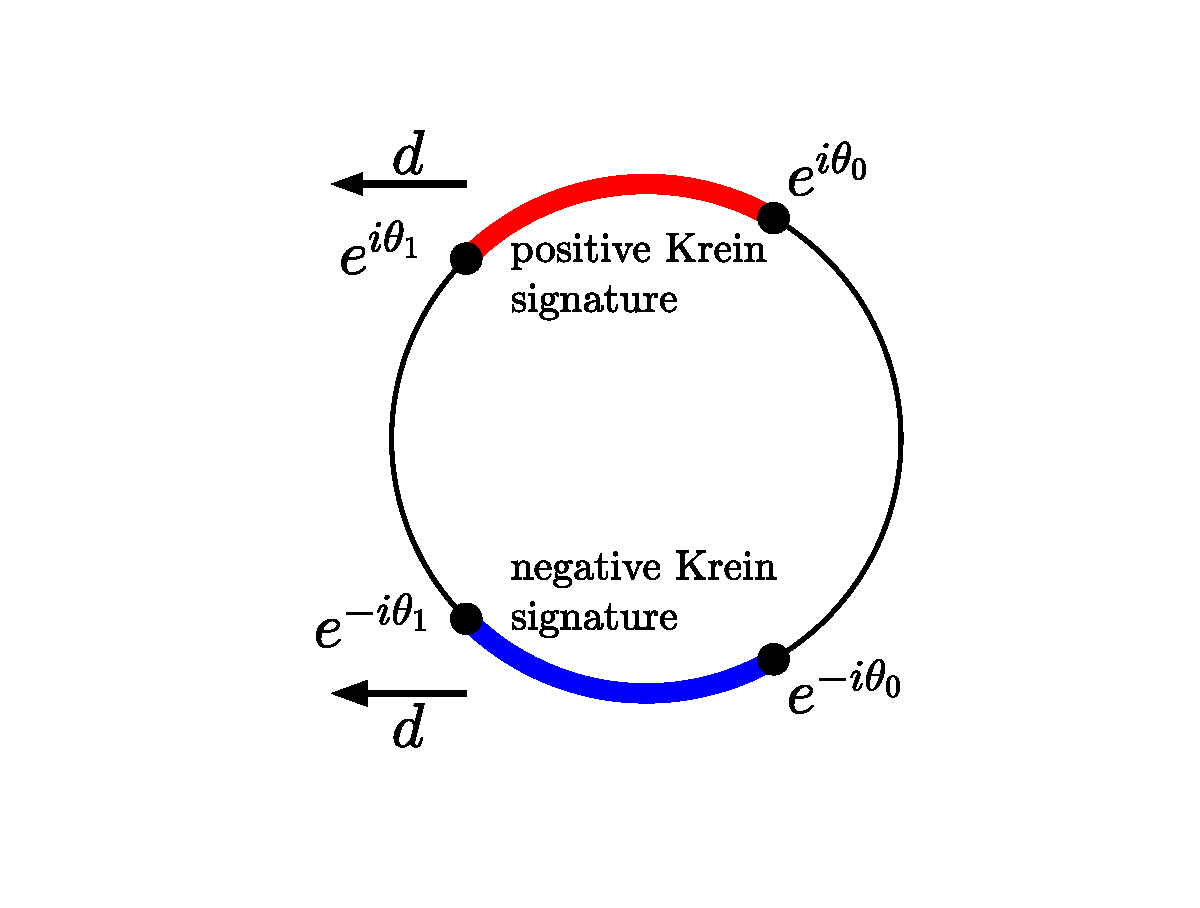
\includegraphics[width=7.5cm]{contspeccartoon1.eps}
	\end{subfigure}
	\begin{subfigure}{0.45\linewidth}
		\caption{}
		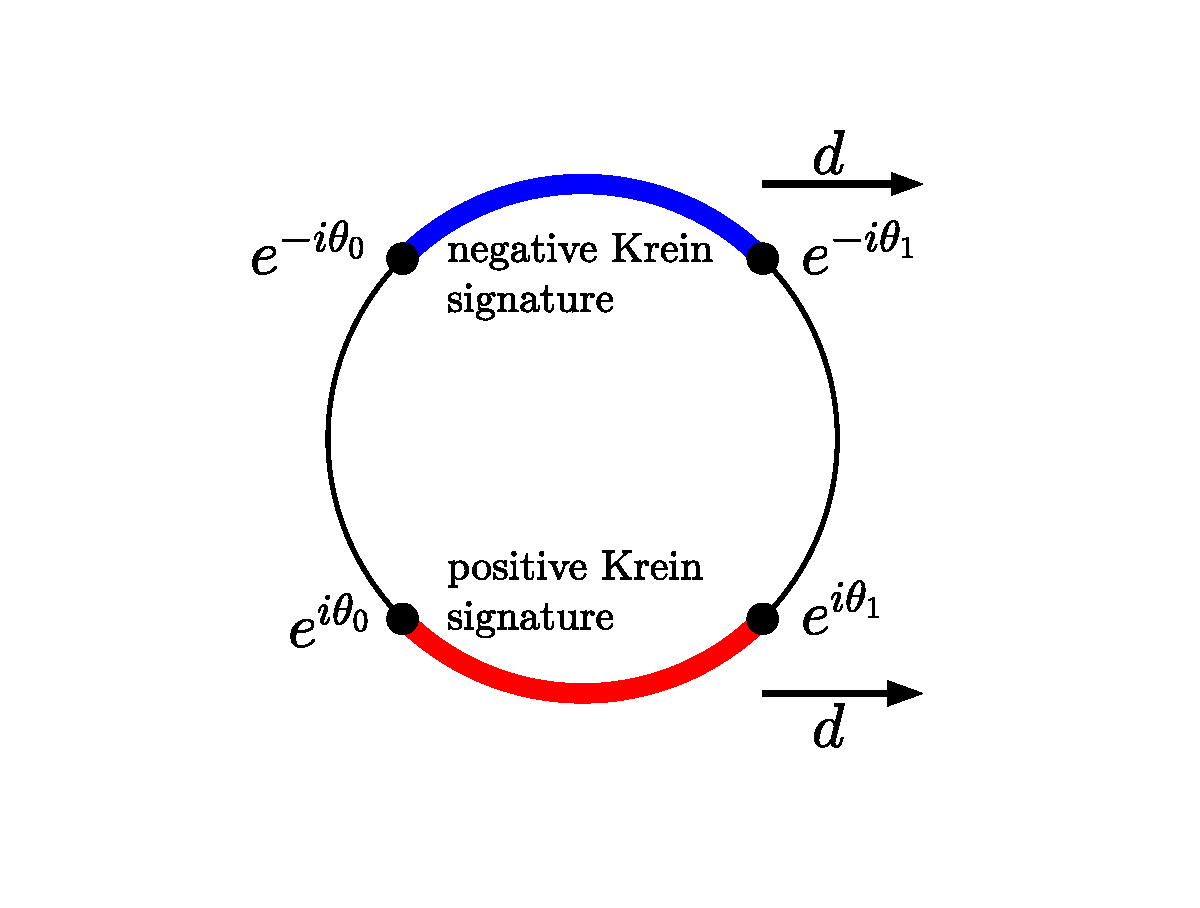
\includegraphics[width=7.5cm]{contspeccartoon2.eps}
	\end{subfigure}
	\end{center}
	\caption{Cartoon showing continuous spectrum bands on the unit circle for $T \in (n \pi, (n+1)\pi)$ with $n$ even (a) and $n$ odd (b). Krein signature of bands is indicated, and bands grow in the direction of the arrow with increasing $d$.}
	\label{fig:bands}
\end{figure}

\subsection{Spatial dynamics}

We now reformulate both the DKG equation \cref{eq:DKG} and the eigenvalue problem \cref{eq:DKGeig} using a spatial dynamics approach, as in \cites{Parker2020,Parker2021}. Let $\uvec(t)$ be a breather solution to \cref{eq:DKG} with period $T$, and define $U(n) = (u(n), \tilde{u}(n)) = ( u_n, u_{n-1} )$. Then equation \cref{eq:DKG} is equivalent to the lattice dynamical system
\begin{equation}\label{eq:dynEq}
U(n+1) = F(U(n)),
\end{equation}
where
\begin{equation}\label{eq:F}
F\begin{pmatrix}u \\ \tilde{u} \end{pmatrix} = 
\begin{pmatrix}2u  + \dfrac{1}{d}f(u) + \dfrac{1}{d} \partial_t^2 u - \tilde{u} \\
u
\end{pmatrix}.
\end{equation}
We note that since $f$ is a odd function, if $U(n)$ is a solution to \cref{eq:dynEq}, then $-U(n)$ is as well. The Floquet eigenvalue problem \cref{eq:DKGeig} can similarly be written as 
\begin{equation}\label{eq:dynEVP}
W(n+1) = \left[ DF(U(n)) + (2 \lambda \partial_t + \lambda^2) B \right] W(n),
\end{equation}
where
\begin{equation}\label{eq:DFU}
DF(U(n)) = \begin{pmatrix}
2 + \dfrac{f'(u(n))}{d} + \dfrac{1}{d}\partial_t^2  & -1 \\ 1 & 0
\end{pmatrix}, \qquad
B = \begin{pmatrix} 1 & 0 \\ 0 & 0 \end{pmatrix}.
\end{equation}
The zero function $U(n) = 0$ is an equilibrium solution to \cref{eq:dynEq}. At this point, the standard procedure (see, for example, \cites{Parker2021,Parker2020,Sandstede1998}) is to consider $U(n)$ as a homoclinic orbit of the equilibrium at 0. The complication here is that for the difference equation \cref{eq:dynEq} to be well-posed, we require $U(n) \in C_\per^\infty([0,T],\R^2)$ for all $n$, rather than just $H^2_\per([0,T], \R^2)$, since each application of $F$ involves differentiating twice with respect to $t$. Since $C_\per^\infty([0,T])$ is not a closed subspace of $L^2([0,T])$, it is not straightforward to adapt the stable manifold theorem and results on exponential dichotomies to this problem, even if $DF(0)$ has the desired spectral properties. As an alternative, we will consider a finite-dimensional approximation, where we project the problem onto a finite-dimensional subspace of $L_\per^2([0,T])$. Roughly, this subspace consists of the first $N$ Fourier modes of the standard basis for $L_\per^2([0,T])$. Although this is a limited result, we note that since we require $U(n)$ to be smooth, its Fourier coefficients will decay exponentially. Since we can take $N$ as large as we like, this should be a very good approximation. In addition, since many of the numerical simulations are performed using Fourier spectral methods, this theory applies directly to that numerical discretization. Before we formulate our approximation, we prove some important results about the spectrum of $DF(0)$.

\subsection{Spectrum of \texorpdfstring{$DF(0)$}{DF(0)}}

The linearization of \cref{eq:dynEq} about the equilibrium at 0 is the constant coefficient linear operator 
\begin{equation}\label{eq:DF0}
DF(0) = \begin{pmatrix}
\dfrac{1}{d}\partial_t^2 + \dfrac{f'(0)}{d} + 2 & -1 \\ 1 & 0
\end{pmatrix},
\end{equation}
which is invertible with inverse
\begin{equation}\label{eq:DF0inv}
DF(0)^{-1} = \begin{pmatrix}
0 & 1 \\ -1 & \dfrac{1}{d}\partial_t^2 + \dfrac{f'(0)}{d} + 2
\end{pmatrix}
\end{equation}
First, we determine the eigenvalues and eigenfunctions of $DF(0)$.

\begin{lemma}\label{lemma:DF0eigs}
The set of eigenvalues of $DF(0)$ is given by $\bigcup_{k \in \Z} \{\lambda_k, \lambda_k^{-1} \}$, where 
\begin{equation}\label{eq:DF0lambdak}
\lambda_k = \frac{1}{2}\left( r_k + \sqrt{r_k^2 - 4} \right), \quad r_k = -\frac{4 k^2 \pi^2}{d T^2} + \frac{f'(0)}{d} + 2.
\end{equation}
For $k \neq 0$, these have algebraic multiplicity 2, since $\lambda_{-k} = \lambda_k$. For each $k \in \Z$, $\{\lambda_k, \lambda_k^{-1} \}$ is either real, or a complex conjugate pair on the unit circle. The eigenfunctions corresponding to $\left\{ \lambda_k, \lambda_k^{-1} \right\}$ are $\left\{ U_k(t), U_k^{-1}(t) \right\}$, which are defined, up to constant multiple, by 
\begin{equation}\label{eq:DF0eigenfns}
\begin{aligned}
U_k(t) &= \begin{pmatrix}v_k(t) \\ \lambda_k^{-1}  v_k(t) \end{pmatrix}, \quad
U_k^{-1}(t) = \begin{pmatrix}v_k(t) \\ \lambda_k v_k(t) \end{pmatrix}, \quad
v_k(t) = \frac{1}{T} \exp\left( i \frac{2 \pi k t}{T} \right).
\end{aligned}
\end{equation}
\end{lemma}
\begin{proof}
Consider the eigenvalue problem $DF(0) U(t) = \lambda U(t)$ on $H^2_\per([0,T],\R^2)$, where $U(t) = (v(t), w(t))^T$. We note that $\lambda = 0$ is not an eigenvalue, since that implies $v = w = 0$. The eigenvalue problem then reduces to the system of equations
\begin{align}\label{eq:DF0EVPsystem}
\left( \frac{1}{d}\partial_t^2 + \frac{f'(0)}{d} + 2 \right) v(t) = \left( \lambda + \frac{1}{\lambda} \right) v(t), \quad
w = \frac{1}{\lambda} v(t).
\end{align}
Letting $r = \lambda + \frac{1}{\lambda}$ and using the periodic boundary conditions $v(T) = v(0)$, the set of solutions to \cref{eq:DF0EVPsystem} is given by
\begin{align}
v_k(t) &= \frac{1}{T} \exp\left( i \frac{2 \pi k t}{T} \right), \quad r_k = -\frac{4 k^2 \pi^2}{d T^2} + \frac{f'(0)}{d} + 2 && k \in \Z,
\end{align}
where the functions $v_k(t)$ have been normalized. The corresponding eigenvalues of $DF(0)$ are then given by $\left\{ \lambda_k, \lambda_k^{-1} \right\}$, where $\lambda_k$ is defined by \cref{eq:DF0lambdak}, and the corresponding eigenfunctions are given by \cref{eq:DF0eigenfns}. The pair $\left\{ \lambda_k, \lambda_k^{-1} \right\}$ is real if $|r_k| \geq 2$, and is complex with modulus 1 if $|r_k| < 2$.
\end{proof}

We note that the spectrum of $DF(0)$ depends on both the coupling parameter $d$ and the period $T$. It follows from \cref{lemma:DF0eigs} that the spectrum of $DF(0)$ is bounded away from the unit circle provided $|r_k| > 2$ for all $k$. The following lemma gives some conditions on $T$ and $d$ to guarantee that this is the case.

\begin{lemma}\label{lemma:DF0hyp}
The spectrum of $DF(0)$ is bounded away from the unit circle if, for a specific nonnegative integer $k$, $T$ and $d$ are chosen so that
\begin{equation}\label{eq:Tdpair}
\frac{2 k \pi}{\sqrt{f'(0)}} < T < \frac{2 (k+1) \pi}{\sqrt{f'(0)}} , \qquad 0 < d < \frac{(k+1)^2\pi^2}{T^2} - \frac{f'(0)}{4}.
\end{equation}
\begin{proof}
Since $f'(0) > 0$, $r_0 = 2 + \frac{1}{d}f'(0) > 2$, and $r_k$ is strictly decreasing in $k$, with $r_k \rightarrow -\infty$ as $k \rightarrow \infty$. Thus $|r_k| > 2$ for all $k$ if $r_k > 2$ and $r_{k+1} < -2$ for some nonnegative integer $k$, from which the conditions \cref{eq:Tdpair} follow.
\end{proof}
\end{lemma}

We take the following assumption on the spectrum of $DF(0)$, which is the analogue to hyperbolicity in the finite-dimensional case.

\begin{hypothesis}\label{hyp:hyp}
The coupling constant $d$ and period $T$ are chosen so that the spectrum of $DF(0)$ is bounded away from the unit circle.
\end{hypothesis}

% Finally, we show that the eigenfunctions of $DF(0)$ are a Hilbert basis for $L^2_\per([0,T],\R^2)$.
% \begin{lemma}\label{lemma:DF0basis}
% Assume \cref{hyp:hyp}. The set of eigenfunctions $\bigcup_{k \in \Z} \{U_k(t) , U_k^{-1}(t) \}$ of $DF(0)$ is a Hilbert basis for $L^2_\per([0,T],\R^2)$, i.e. every function $Y(t) \in L^2_\per([0,T],\R^2)$ can be written uniquely as
% \begin{equation}\label{eq:yinDF0basis}
% Y(t) = \sum_{k \in \Z} a_k U_k(t) + \sum_{k \in \Z} b_k U^{-1}_k(t),
% \end{equation}
% where $a_k, b_k \in \C$ and the sum converges for all $Y(t)$.
% \begin{proof}
% Letting $v_k(t) = \frac{1}{T} \exp\left( i \frac{2 \pi k t}{T} \right)$, the set $\{ v_k(t) : k \in \Z \}$ is an orthonormal basis for $L^2_\per([0,T],\R)$. It follows that the set $\bigcup_{k \in \Z} \{Z^1_k(t) , Z^2_k(t) \}$ is an orthonormal basis for $L^2_\per([0,T],\R^2)$, where $Z^1_k(t) = (v_k(t), 0)^T$ and $Z^2_k(t) = (0, v_k(t))^T$. Therefore, there exist unique scalars $c_k, d_k \in \C$ such that
% \begin{equation*}
% Y(t) = \sum_{k \in \Z} c_k Z^1_k(t) + \sum_{k \in \Z} d_k Z^2_k(t),
% \end{equation*}
% and the sum converges for all $Y(t)$. Equation \cref{eq:yinDF0basis} follows by taking
% \[
% a_k = \frac{1}{\lambda_k^2 - 1}\left(-c_k + \lambda_k d_k \right), \quad
% b_k = \frac{1}{\lambda_k^2 - 1}\left( \lambda_k^2 c_k - \lambda_k d_k \right),
% \]
% where $\lambda_k$ is defined in \cref{eq:DF0lambdak}, and $\lambda_k^2 \neq 1$ by \cref{hyp:hyp}.
% \end{proof}
% \end{lemma}

\section{Finite dimensional approximation}

In this section, we define our finite dimensional approximation for \cref{eq:dynEq}. For $M \geq 1$, let 
\begin{equation}\label{eq:XM}
X_M = \spn\left\{ \bigcup_{k = -M}^M v_k(t) \right\}, \qquad
v_k(t) = \frac{1}{T} \exp\left( i \frac{2 \pi k t}{T} \right)
\end{equation}
be the $(2M+1)$-dimensional subspace of $L_\per^2([0,T])$ spanned by the Fourier basis functions with wavenumber $|k| \leq M$, and let $P_M: L_\per^2([0,T]) \rightarrow X_M$, defined by
\begin{equation}\label{eq:PM}
P_M u(t) = \sum_{k=-M}^M \langle u, v_k \rangle_{L^2([0,T])} v_k(t)
= \sum_{k=-M}^M \left( \int_0^T u(s) \overline{v_k(s)} ds \right) v_k(t)
\end{equation}
be the corresponding projection operator. In addition, let $X_{M,e}$ be the $(M+1)$-dimensional subspace of $X_M$ comprising functions which are even in $t$, i.e.
\begin{equation}
X_{M,e} = \left\{ f \in X_M : f(-t) = f(t) \text{ for all }t \in \R \right\}.
\end{equation}

For $M \geq 1$, we define the approximation of the discrete Klein-Gordon equation \cref{eq:DKG} on $\ell^2(\Z, X_M)$ by
\begin{equation}\label{eq:DKGapprox}
\begin{aligned}
\ddot{u}_n &= d (\Delta_2 u)_n - g(u_n) && \qquad u_n \in X_M,
\end{aligned}
\end{equation}
where $g: X_M \rightarrow X_M$ is defined by $g(u) = P_M f(u)$. When $u = 0$, $g(0) = P_M f(0) = 0$, and $g'(0) = P_M f'(0) = f'(0)$, since $f'(0)$ is a constant function, which is in $X_M$ for all $M$.
Furthermore, since $f$ is an odd function, $g$ is as well. In general, it not the case that $P_M f(u) = f(P_M u)$, thus we cannot simply obtain a solution to \cref{eq:DKGapprox} by projecting a solution of \cref{eq:DKG} onto $X_M$. However, since the Fourier coefficients of a smooth, $T$-periodic function $u(t)$ decay exponentially, equation \cref{eq:DKGapprox} should be a reasonable approximation to \cref{eq:DKG} for large $M$. Linearization of \cref{eq:DKGapprox} about a solution $\uvec \in \ell^2(\Z, X_M)$ yields the eigenvalue problem
\begin{equation}\label{eq:DKGMeig}
\begin{aligned}
d (\Delta_2 w)_n - g'(u_n)w_n - \ddot{w}_n = 2 \lambda \dot{w}_n + \lambda^2 w_n,
\end{aligned}
\end{equation}
which we write as
\begin{equation}\label{eq:DKGMeigL}
\calL_M(\uvec)\wvec = (2 \lambda \partial_t + \lambda^2 )\wvec,
\end{equation} 
where $\calL_M(\uvec)$ is the linear operator on $\ell^2(\Z, X_M)$ defined by the LHS of \cref{eq:DKGMeigL}. As in \cref{sec:DKGlinear}, $\calL_M(\uvec) \dot{\uvec} = 0$, and there exists a solution $\yvec$ to $\calL_M(\uvec) \yvec = 2 \ddot{\uvec}$, where $\yvec = \omega \partial_\omega \uvec$ and $\omega = 2 \pi / T$.

Reformulating \cref{eq:DKGapprox} from a spatial dynamics perspective yields the discrete dynamical system on $X_M^2$
\begin{align}\label{eq:dynEqM}
U(n+1) &= F_M(U(n)) && U(n) \in X_M^2,
\end{align}
where
\begin{equation}\label{eq:FM}
F_M\begin{pmatrix}u \\ \tilde{u} \end{pmatrix} = 
\begin{pmatrix}2u  + \dfrac{1}{d}g(u) + \dfrac{1}{d} \partial_t^2 u - \tilde{u} \\
u
\end{pmatrix}
\end{equation}
Since $F_M(-U) = -F_M(U)$, it follows that if $U(n)$ is a solution to \cref{eq:dynEqM}, so is $-U(n)$. Similarly, the eigenvalue problem \cref{eq:DKGMeig} can be reformulated as
\begin{equation}\label{eq:dynEVPM}
W(n+1) = \left[ DF_M(U(n)) + (2 \lambda \partial_t + \lambda^2) B \right] W(n),
\end{equation}
where $B$ is defined in \cref{eq:DFU}. Since $g'(0) = f'(0)$, the linear operator $DF_M(0)$ on $X_M^2$ is also given by \cref{eq:DF0}. 

Finally, let $\{\tau(s) : s \in \R\}$ be the one-parameter group of unitary translation operators on $X_M^2$, defined by $[\tau(s)]U(\cdot) = U(\cdot - s)$, which has infinitesimal generator $\tau'(0) = \partial_t$. We note that this group is well-defined on $X_M^2$, since 
\[
\tau(s) v_k(t) 
\frac{1}{T} \exp\left( i \frac{2 \pi k (t-s)}{T}\right) 
= \exp\left( -i \frac{2 \pi k s}{T} \right) \frac{1}{T} \exp\left( i \frac{2 \pi k t}{T}\right) 
= \exp\left( -i \frac{2 \pi k s}{T} \right) v_k(t),
\]
i.e. the group action multiplies a basis element by a constant. In fact, the eigenvalue of \cref{eq:DKGMeig} at 0 is a result of this translational symmetry. The function $F_M$ from \cref{eq:dynEqM} (as well as $F$ from the full system \cref{eq:dynEq}) commutes with this one-parameter group, i.e. $F(\tau(s) U) = \tau(s) F(U)$. It is cruicial to note that this symmetry is lost if we consider the problem \cref{eq:dynEqM} on $X_{M,e}^2$, since the space of even functions is not translation invariant. 

\section{Multi-breathers}

Our strategy will be to first prove that multi-breathers exist on the subspace $X_{M,e}^2$ of even functions. Since there is no translational symmetry, the stable and unstable manifolds of the origin will intersect transversely, which greatly simplifies the analysis. This parallels the restriction in \cite{Pelinovsky2012} to breathers which are even in $t$, and is consistent with the odd symmetry of the nonlinearity $f$. 
Once that is accomplished, we will return to the full space $X_{M}^2$ for the eigenvalue problem, and use Lin's method as in \cites{Parker2021,Parker2020,Sandstede1998} to construct interaction eigenfunctions as piecewise linear combinations of the eigenfunction corresponding to translation symmetry. This technique is similar to the one we employed in \cite{Parker2020} for DNLS, where, to prove the existence of multi-pulses, we removed the gauge symmetry by restricting the problem to real-valued solutions.

\subsection{Primary breather}

To accomplish this, we will take the existence of a primary, single-site breather as a hypothesis. 
Fix $d$ and $T$ such that \cref{hyp:hyp} holds. First, we consider the system \cref{eq:dynEqM} on $X_{M,e}^2$. By \cref{lemma:DF0eigs}, the $2M+2$ eigenvalues of $DF_M(0)$ on $X_{M,e}^2$ are given by $S_M = \bigcup_{k=0}^M \{\lambda_k, \lambda_k^{-1} \}$, where these are defined in the statement of \cref{lemma:DF0eigs}. By \cref{hyp:hyp}, the spectrum of $DF_M(0)$ is real and does not intersect the unit circle, thus 0 is a hyperbolic equilibrium point of \cref{eq:dynEqM}. Define the stable and unstable subsets of the spectrum of $DF_M(0)$ by
\[
S_M^s = \{ \lambda \in S_M : |\lambda| < 1\}, \qquad S_M^u = \{ \lambda \in S_M : |\lambda| > 1\}.
\]
By symmetry, $|S_M^s| = |S_M^u| = M+1$. Define
\begin{equation}\label{eq:defrM}
r_M = \min \{ |\lambda| : \lambda \in S_M^u, |\lambda| > 1 \}.
\end{equation}
Since $X_{M,e}^2$ is finite-dimensional, the stable manifold holds. For each $M \geq 1$, let $W_{M,e}^s(0)$ and $W_{M,e}^u(0)$ be the $(M+1)$-dimensional stable and unstable manifolds of the equilibrium at 0, which are subsets of $X_{M,e}^2$. A breather solution to \cref{eq:dynEqM} is a homoclinic orbit which lies in the intersection of the stable and unstable manifolds. We take the existence of such a solution as a hypothesis.

\begin{hypothesis}\label{hyp:breather}
Let $d$ and $T$ be chosen according to \cref{hyp:hyp}. There exists a positive integer $M_0$ such that for all $M \geq M_0$, the stable and unstable manifolds $W_{M,e}^s(0)$ and $W_{M,e}^u(0)$ intersect transversely in $X_{M,e}^2$ in a homoclinic orbit $Q_M(n) = (q(n), \tilde{q}(n))^T = (q_n, q_{n-1})^T$. 
\end{hypothesis}
The first component $q_n$ is a breather solution to \cref{eq:DKGapprox}. As a consequence of the stable manifold theorem, we have the estimate 
\begin{equation}\label{eq:U1decayest}
\|Q_M(n)\|_{L^2_\per([0,T])} \leq C r_M^{-|n|}.
\end{equation}

We now consider \cref{eq:dynEqM} on $X_M^2$. The spectrum of $DF(0)$ on $X_M^2$ is exactly the same as that on $X_{M,e}^2$, except the eigenvalues corresponding to $k = 1, \dots, M$ have multiplicity of 2. It follows that 0 is also a hyperbolic equilibrium of \cref{eq:dynEqM} on $X_M^2$. Let $W_M^s(0)$ and $W_M^u(0)$ be the $(2M+1)$-dimensional stable and unstable manifolds of the equilibrium at 0, which this time are subsets of $X_M^2$. For $M \geq M_0$, $Q_M(n)$ is also a homoclinic orbit connecting these stable and unstable manifolds. In the next hypothesis, we assume that this intersection is non-degenerate.

\begin{hypothesis}\label{hyp:breathernondegen}
Let $d$ and $T$ be chosen according to \cref{hyp:hyp}, and let $M_0$ and $Q_M(n)$ be as in \cref{hyp:breather}. Then for all $M \geq M_0$, the stable and unstable manifolds $W_M^s(0)$ and $W_M^u(0)$ have a one-dimensional intersection in $Q_M(n)$.
\end{hypothesis}

The variational equation is the linearization of \cref{eq:dynEqM} on $X_M^2$ about the homoclinic orbit solution $Q_M(n)$, which is given by
\begin{equation}\label{eq:vareq}
\begin{aligned}
W(n+1) &= DF_M(Q_M(n)) W(n) && W(n) \in X_M^2.
\end{aligned}
\end{equation}
Since the tangent spaces of $W_M^s(0)$ and $W_M^u(0)$ have a one-dimensional intersection by \cref{hyp:breathernondegen}, it follows that $\dot{Q}_M(n) = (\dot{q}_n, \dot{q}_{n-1})$ is the unique, bounded solution to \cref{eq:vareq}, up to scalar multiples. ($\dot{Q}_M(n)$ is not a solution to \cref{eq:vareq} on $X_{M,e}^2$, since it is an odd function). We can thus decompose the tangent spaces to $W_M^u(0)$ and $W_M^s(0)$ at $U_M^1(0)$ as
\begin{equation}\label{eq:TWdecomp}
T_{Q_M(0)}W^u_M(0) = \R \dot{Q}_M(0) \oplus Y_M^-, \qquad  
T_{Q_M(0)}W^s_M(0) = \R \dot{Q}_M(0) \oplus Y_M^+,
\end{equation}
where $\dim Y_M^- = \dim Y_M^+ = 2M$. In addition, the adjoint variational equation
\begin{equation}\label{eq:adjvareq}
Z(n) = DF_M(Q_M(n))^* Z(n+1)
\end{equation}
has a unique bounded solution, given by
\begin{equation}\label{eq:Z1}
Z_M(n) = (-\dot{q}_{n-1}, \dot{q}_n)^T,
\end{equation}
and $Z_M(0) \perp \R \dot{Q}_M(0) \oplus Y_M^- \oplus Y_M^+$ by \cite{Parker2020}*{Lemma 1}. We can thus decompose $X_M^2$ as
\begin{equation}\label{eq:Xdecomp}
X_M^2= \R \dot{Q}_M(0) \oplus Y_M^- \oplus Y_M^+ \oplus \R Z_M(0).
\end{equation}

\subsection{Existence}

We construct a multi-breather on $X_{M,e}$ by splicing together multiple copies of the primary breather $Q_M(n)$ in a chain. We characterize a multi-breather in the following way. Let $m > 1$ be the total number of copies of the primary breather in the chain. Let $N_i$ ($i = 1, \dots, m-1$) be the distances (in lattice points) between the center point of each breather. We seek to construct a solution $U(n)$ which can be written piecewise in the form
\begin{equation}\label{eq:Upiecewise}
\begin{aligned}
U_i^-(n) &= \sigma_i Q_M(n) + \tilde{U}_i^-(n) && n \in [-N_{i-1}^-, 0] && \quad i = 1, \dots, m\\
U_i^+(n) &= \sigma_i Q_M(n) + \tilde{U}_i^+(n) && n \in [0, N_i^+] && \quad i = 1, \dots, m,
\end{aligned}
\end{equation}
where $\sigma_i \in \{1, -1\}$ represents the orientation of each copy of the primary breather, $N_i^+ = \lfloor \frac{N_i}{2} \rfloor$, $N_i^- = N_i - N_i^+$, and $N_0^- = N_m^+ = \infty$. Adjacent copies of the primary breather are in-phase if $\sigma_i \sigma_{i+1} = 1$, or out-of-phase if $\sigma_i \sigma_{i+1} = -1$. (As in \cite{Pelinovsky2012}, other phase relations are not considered here). The functions $\tilde{U}_i^\pm$ in \cref{eq:Upiecewise} are remainder terms, which will be small. We also define the characteristic distance
\begin{equation}\label{defN}
N = \frac{1}{2} \min\{ N_i \},
\end{equation}
which will be used in the estimates of the remainder terms $\tilde{U}_i^\pm$. The individual pieces $U_i^\pm(n)$ are joined together end-to-end as in \cites{Sandstede1998,Knobloch2000,Parker2020,Parker2021} to create the multi-breather $U(n)$, which can be written in piecewise form as
\begin{equation}
\begin{aligned}
U(n) &= \begin{cases}
U_i^-\left( n - \sum_{j=1}^{i-1}N_j \right) & \sum_{j=1}^{i-1}N_j - N_{i-1}^- + 1 \leq n \leq \sum_{j=1}^{i-1}N_j \\
U_i^+\left( n - \sum_{j=1}^{i-1}N_j \right) & \sum_{j=1}^{i-1}N_j + 1 \leq n \leq \sum_{j=1}^{i-1}N_j + N_i^+
\end{cases}
&& i = 1, \dots, m,
\end{aligned}
\end{equation}
where we define $\sum_{j=1}^0 N_j = 0$. We have the following existence theorem concerning the existence of multi-breathers on $X_{M,e}$. 

\begin{theorem}\label{th:multibreathers}
Assume \cref{hyp:hyp} and \cref{hyp:breather}, and let $M \geq M_0$, where $M_0$ is defined in \cref{hyp:breather}. Then there exists a positive integer $N_0$ with the following property. For all $m > 1$ and distances $N_i \geq N_0$, there exists a unique solution $U(n)$ which comprises, to leading order, $m$ sequential copies of the primary breather, and can be written piecewise in the form \cref{eq:Upiecewise}. For the remainder terms $\tilde{U}_i^\pm(n)$, we have the estimates
\begin{equation}\label{eq:Uestimates}
\begin{aligned}
\tilde{U}_i^+(N_i^+) &= \sigma_{i+1} Q_M(-N_i^-) + \mathcal{O}(r_M^{-2N}) \\
\tilde{U}_{i+1}^-(-N_i^-) &= \sigma_{i} Q_M(N_i^+) + \mathcal{O}(r_M^{-2N}) \\ 
\| \tilde{U}_i^-(n)\|_{X_M} &\leq C r_M^{-N_{i-1}^-} r_M^{-(N_{i-1}^- + n)} && \qquad n = 2, \dots, m\\
\|\tilde{U}_i^+(n) \|_{X_M} &\leq C r_M^{-N_i^+} r_M^{-(N_i^+ - n)} && \qquad n = 1, \dots, m-1 \\
\| \tilde{U}_1^-(n)\|_{X_M} &\leq C r_M^{-2N} r_M^{n} \\
\|\tilde{U}_m^+(n) \|_{X_M} &\leq C r_M^{-2N} r_M^{-n},
\end{aligned}
\end{equation}
which hold as well for derivatives of $\tilde{U}_i^\pm(n)$.
\begin{proof}
The proof is a straightforward adaptation of the proofs of theorems 1 and 3 in \cite{Parker2020}, and is very similar to the proof of \cite{Parker2021}*{Theorem 1}. Since the stable and unstable manifolds $W_{M,e}^s(0)$ and $W_{M,e}^u(0)$ intersect transversely in $X_{M,e}$, the implementation of Lin's method does not involve jump conditions.
\end{proof}
\end{theorem}

\subsection{Spectral stability}

For a multi-breather consisting of $m$ components, as long as the individual copies of the primary breather are sufficiently well separated, there will be $2(m-1)$ eigenvalues in spectrum of \cref{eq:DKGMeig}, i.e. one pair per additional copy of the primary breather, which will be located near the origin. We call these interaction eigenvalues, since they result from nonlinear interactions between the tails of adjacent copies of the primary breather. (These are called internal modes in \cite{cuevas-maraver2016}; since we will see other internal modes when we perform numerical experiments in \cref{sec:numerics}, we will reserve the term interaction eigenvalues for these specific internal modes).
As in \cites{Parker2020,Sandstede1998}, we locate these eigenvalues by using Lin's method to construct the corresponding eigenfunctions. We note that this theorem gives the Floquet exponents $\lambda$, which are the eigenvalues of \cref{eq:DKGMeig}. The Floquet multipliers $\mu$ are related to these by $\mu = e^{\lambda T}$. The proof is given in \cref{app:specproof}.

\begin{theorem}\label{th:spectrum}
Assume \cref{hyp:hyp}, \cref{hyp:breather}, and \cref{hyp:breathernondegen}, and let $M \geq M_0$, where $M_0$ is defined in \cref{hyp:breather}. Let $Q_M(n) = (q_n, q_{n-1})$ be the primary breather solution from \cref{hyp:breather}, and let $Y(n) = (y_n, y_{n-1}) = \omega \partial_\omega Q_M(n)$.
Let $U(n)$ be an $m$-component multi-breather constructed as in \cref{th:multibreathers} with distances $N_i$ and orientation parameters $\sigma_i$. Then there exists $\delta > 0$ with the following property. There exists a bounded, nonzero solution $W(n)$ of the eigenvalue problem \cref{eq:dynEVPM} on $X_M^2$ for $|\lambda| < \delta$ if and only if $E(\lambda) = 0$, where
\begin{equation}\label{Elambda}
E(\lambda) = \det\left(A + \frac{1}{d}M \lambda^2 I + R(\lambda)\right).
\end{equation}
$A$ is the tri-diagonal $m \times m$ matrix
\begin{align}\label{eq:matrixA}
A &= \begin{pmatrix}
-a_1 & a_1 & & & \\
-\tilde{a}_1 & \tilde{a}_1 - a_2 & a_2 \\
& -\tilde{a}_2 & \tilde{a}_2 - a_3 & a_3 \\
& \ddots & & \ddots \\
& & & -\tilde{a}_{m-1} & \tilde{a}_{m-1}  \\
\end{pmatrix},
\end{align}
with
\begin{equation}\label{eq:ai}
\begin{aligned}
a_i &= \sigma_i \sigma_{i+1} \int_0^T \left( \dot{q}_{N_i^+}\dot{q}_{-N_i^- - 1} 
- \dot{q}_{N_i^+ - 1}\dot{q}_{-N_i^-} \right) dt \\
\tilde{a}_i &= \sigma_i \sigma_{i+1} \int_0^T \left( \dot{q}_{-N_i^-} \dot{q}_{N_i^+ - 1} 
- \dot{q}_{-N_i^- - 1}\dot{q}_{N_i^+} \right) dt,
\end{aligned}
\end{equation}
\begin{align}\label{eq:M}
M =
\sum_{n = -\infty}^\infty \int_0^T \left( \dot{q}_n^2 + 2 \dot{y}_n \dot{q}_n \right) dt,
\end{align}
and the remainder term has uniform bound
\begin{equation}\label{eq:Rbound}
\|R(\lambda)(c)\|_{X_M^2} \leq C \left( (r_M^{-N} + |\lambda|)^3\right).
\end{equation}
\end{theorem}

\begin{remark}If the primary breather $Q_M = (q_n, q_{n-1})$ has the even spatial symmetry $q_{-n} = q_n$, then the matrix $A$ in \cref{th:spectrum} simplifies to
\begin{align}\label{matrixAsymm}
A &= \begin{pmatrix}
-a_1 & a_1 & & & \\
a_1 & -a_1 - a_2 & a_2 \\
& a_2 & -a_2 - a_3 & a_3 \\
& \ddots & & \ddots \\
& & & a_{m-1} & -a_{m-1}  \\
\end{pmatrix},
\end{align}
with
\begin{align*}
a_i &= \begin{cases}
\sigma_i \sigma_{i+1} \int_0^T \dot{q}_{\frac{N_i}{2}}\left( \dot{q}_{\frac{N_i}{2}+1} - \dot{q}_{\frac{N_i}{2}-1}\right) dt & N_i \text{ even} \\
\sigma_i \sigma_{i+1} \int_0^T \left( \dot{q}_{\frac{N_i-1}{2}}\dot{q}_{\frac{N_i+3}{2}} - \dot{q}_{\frac{N_i+1}{2}}\dot{q}_{\frac{N_i-3}{2}} \right) dt & N_i \text{ odd}
\end{cases}
\end{align*}
In this case, the matrix $A$ has one eigenvalue at 0, and the remaining $(m-1)$ eigenvalues $\{\mu_1, \dots, \mu_{m-1}\}$ are real and distinct (see the proof of \cite{Parker2020}*{Theorem 5}). It follows from \cref{th:spectrum} that, as long as the continuous spectrum does not interfere, there are $(m-1)$ pairs of interaction eigenvalues, given by 
\begin{align}\label{eq:inteigs}
\lambda_j &= \pm \sqrt{-\frac{d \mu_j}{M}} + \mathcal{O}(r^{-2N}) && j = 1, \dots, m-1,
\end{align}
and these are either real or imaginary by Hamiltonian symmetry. For a double breather ($m = 2$), the pair of interaction eigenvalues is given by
\begin{align}\label{eq:inteigsdouble}
\lambda &= \sqrt{\frac{2 a_1 d}{M}} + \mathcal{O}(r^{-2N}).
\end{align}
\end{remark}

\begin{remark}
Substituting $y_n = \omega \partial_\omega q_n$, we can write \cref{eq:M} as 
\begin{align}\label{eq:M2}
M =
\sum_{n = -\infty}^\infty \int_0^T \dot{q}_n \left( 2 \omega \partial_\omega \dot{q}_n + \dot{q}_n \right) dt,
\end{align}
which is the solvability condition from \cite{kevrekidis2016}. Integrating by parts, we can also write \cref{eq:M} as 
\begin{align}\label{eq:M3}
M =
\sum_{n = -\infty}^\infty \int_0^T \left( \dot{q}_n^2 - 2 y_n \ddot{q}_n \right) dt =
\sum_{n = -\infty}^\infty \int_0^T \left( \dot{q}_n^2 - 2 (\partial_\omega q_n) \ddot{q}_n \right) dt.
\end{align}
\end{remark}

\section{Numerical results}\label{sec:numerics}

We construct both the primary breather and multi-breathers by numerical parameter continuation from the AC limit using the software package AUTO \cite{auto07p}. To do this, we first choose an energy level $E$, from which we compute the period $T$ using \cref{eq:ET}, and then determine the AC breather solution $\phi(t)$ by solving \cref{eq:singlesiteAC} with the initial conditions given in \cref{sec:DKGbreather}. For the initial condition at $d = 0$, we take $u_k(t) = \phi(t)$ at a finite set of lattice points, and $u_k = 0$ everywhere else. For the parameter continuation, we use the equation
\begin{equation}\label{eq:HformAUTO}
\frac{d}{dt}\begin{pmatrix} u_n \\ v_n \end{pmatrix} = 
\begin{pmatrix} 0 & 1 \\ -1 & 0 \end{pmatrix}\begin{pmatrix} \partial \calH / \partial u_n \\ \partial \calH / \partial v_n \end{pmatrix} + 
\epsilon \begin{pmatrix} \partial \calH / \partial u_n \\ \partial \calH / \partial v_n \end{pmatrix},
\end{equation}
where $\calH$ is the Hamiltonian defined by \cref{eq:H} and $\epsilon$ is a small parameter used to break the Hamiltonian structure. To avoid continuing in the direction of translation symmetry, we add the phase condition
\[
\langle \dot{u_k}^\text{old}, u_k - u_k^\text{old} \rangle =
\int_0^T v_k^\text{old}( u_k - u_k^\text{old}) dt,
\]
where $u_k^\text{old}$ refers to the function at the previous continuation step. The index $k$ is chosen to be one of the lattice points at which the initial condition is $\phi(t)$. We approximate the integer lattice with a finite lattice of length $2L+1$, numbered from $-L$ to $L$, and we take Dirichlet boundary conditions at the ends of the lattice, i.e. $u_{L+1} = u_{-L-1} = 0$. Thus equation \cref{eq:Hform} becomes an ODE in $4L+2$ dimensions, with periodic boundary conditions imposed on each variable. Once a breather solution has been found, its Floquet spectrum is found numerically by using Matlab's numerical eigenvalue solver \texttt{eig} to compute the eigenvalues of the monodromy operator.

\subsection{Discrete sine-Gordon equation}

We first consider the discrete sine-Gordon equation, where the nonlinearity is $f(u) = \sin u$. For all of the plots in the section, we use a lattice size $L = 15$, the energy at AC limit is $E = 0.25$, and the period is $T = 7.91$. We note that $2 \pi < T < 3 \pi$, thus the upper continuous spectrum band has positive Krein signature, and the lower band has negative Krein signature (\cref{fig:bands}, left).
\cref{fig:singlea} shows the primary breather solution for $d = 0.25$ at $t = 0$, which is symmetric on the spatial lattice. The corresponding Floquet spectrum is shown in \cref{fig:singleb}. There is a single Floquet multiplier (with multiplicity 2) at 1, which is from translation symmetry. The continuous spectrum bands are a discrete set of points, which is a result of the spatial discretization, and have merged into a single band by this value of $d$. \cref{fig:singlec} shows the exponential decay of the breather with increasing $n$; \cref{fig:singled} shows the relative error of this decay rate compared to $r_M$, which is defined in \cref{eq:defrM}. The exponential decay of the Fourier frequencies (in $t$) of the primary breather is shown in \cref{fig:freqdecay}. As expected, since the breather is even in $t$, only even frequencies are represented in the frequency spectrum. Furthermore, the scaled amplitudes for all frequencies $k\geq 20$ are below $10^{-10}$, suggesting that the finite dimensional approximation is reasonable.

\begin{figure}
	\begin{center}
	\begin{subfigure}{0.45\linewidth}
		\caption{}
		\includegraphics[width=7.5cm]{singleun0.eps}
		\label{fig:singlea}
	\end{subfigure}
	\begin{subfigure}{0.45\linewidth}
		\caption{}
		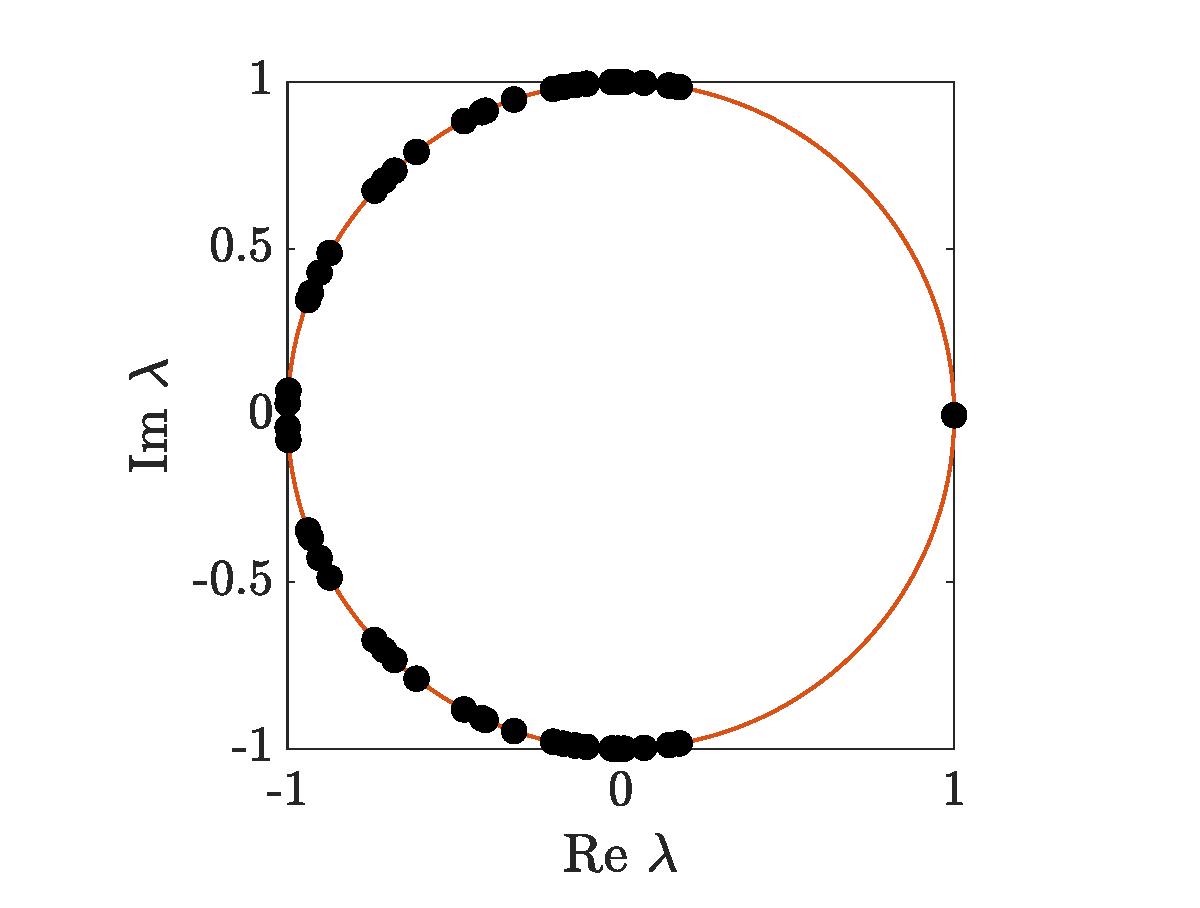
\includegraphics[width=7.5cm]{singlespec.eps}
		\label{fig:singleb}
	\end{subfigure}
	\begin{subfigure}{0.45\linewidth}
		\caption{}
		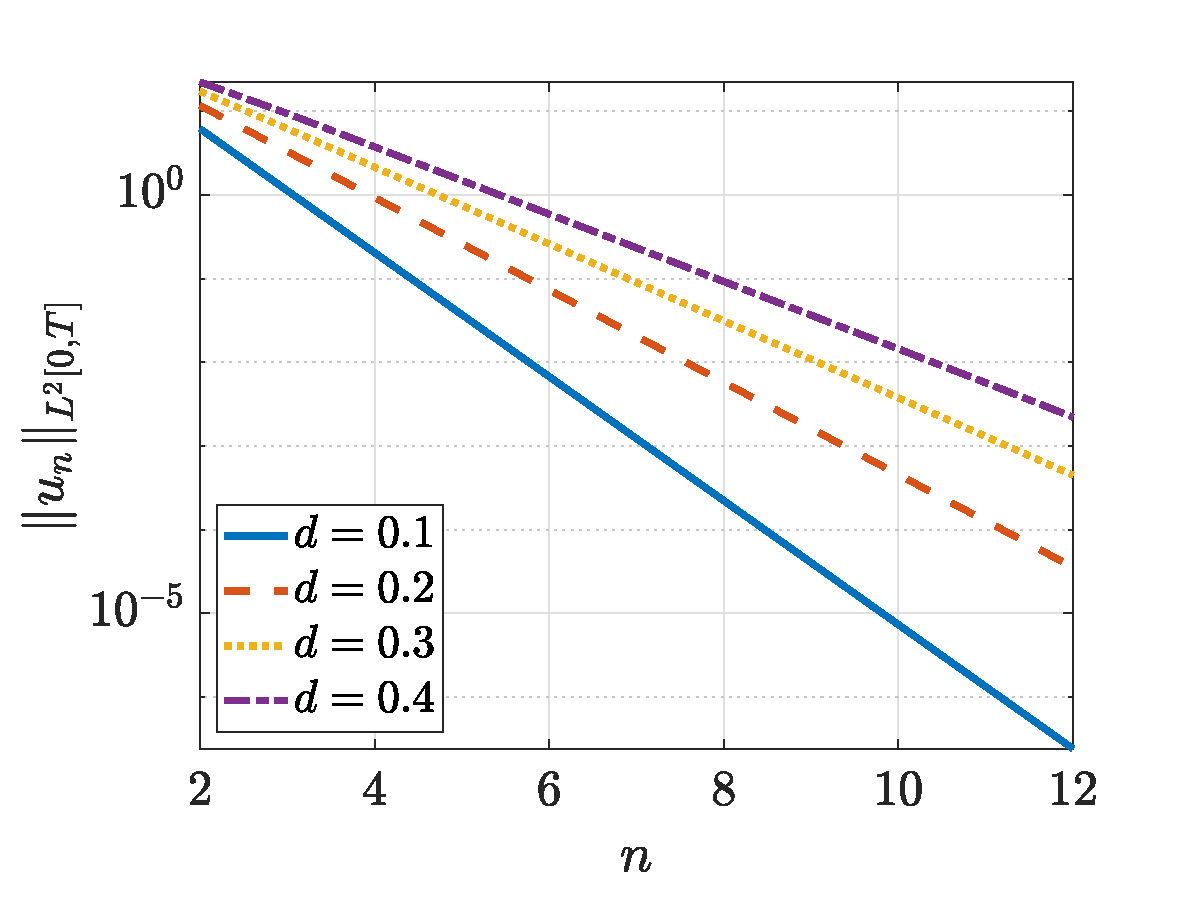
\includegraphics[width=7.5cm]{singledecay.eps}
		\label{fig:singlec}
	\end{subfigure}
	\begin{subfigure}{0.45\linewidth}
		\caption{}
		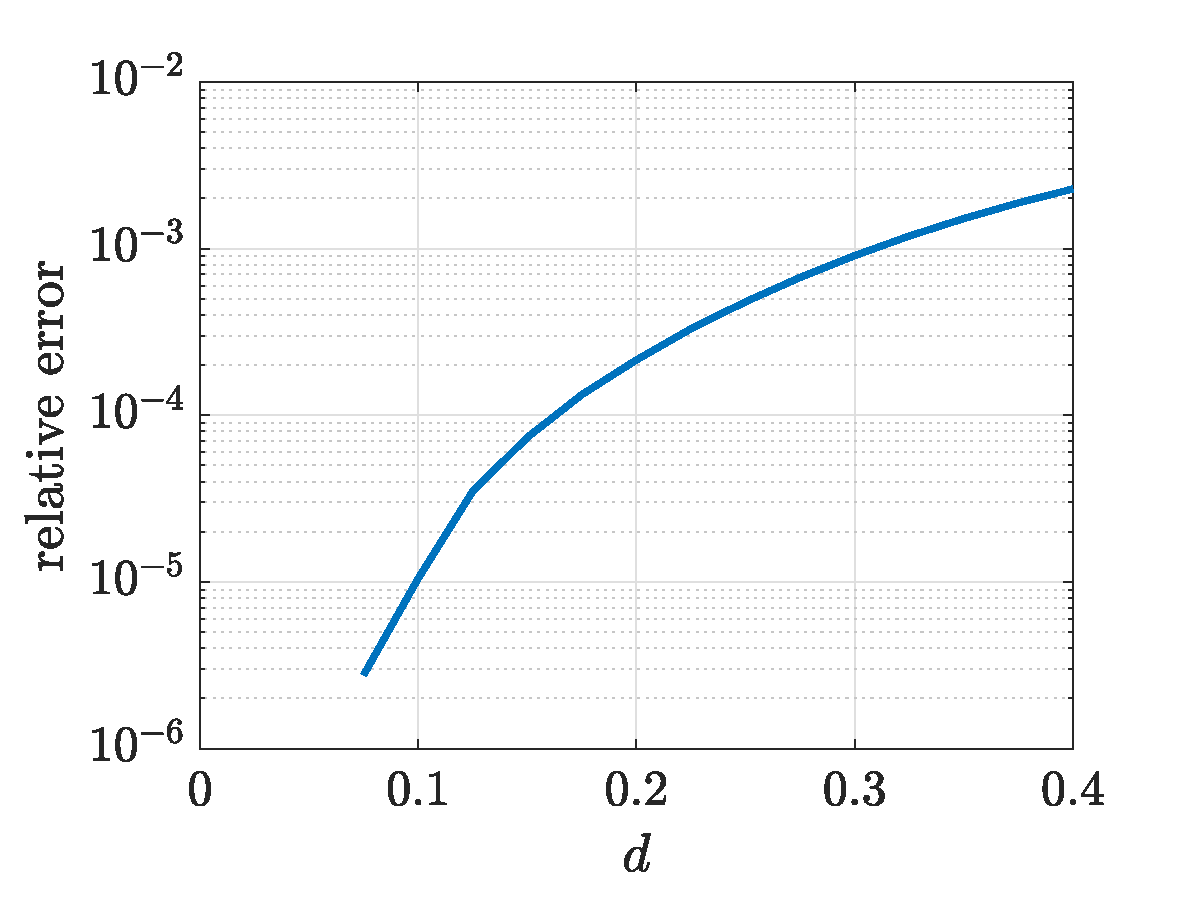
\includegraphics[width=7.5cm]{singledecayerror.eps}
		\label{fig:singled}
	\end{subfigure}
	\end{center}
	\caption{(a) Initial condition $u_n(0)$, and (b) Floquet spectrum, for primary breather for $d = 0.25$. (c) Semilog plot showing exponential decay rate of $L^2$ norm of breather solution with increasing $n$ for varying $d$. (d) Relative error in exponential decay rate. }
	\label{fig:single}
\end{figure}

\begin{figure}
	\begin{center}
	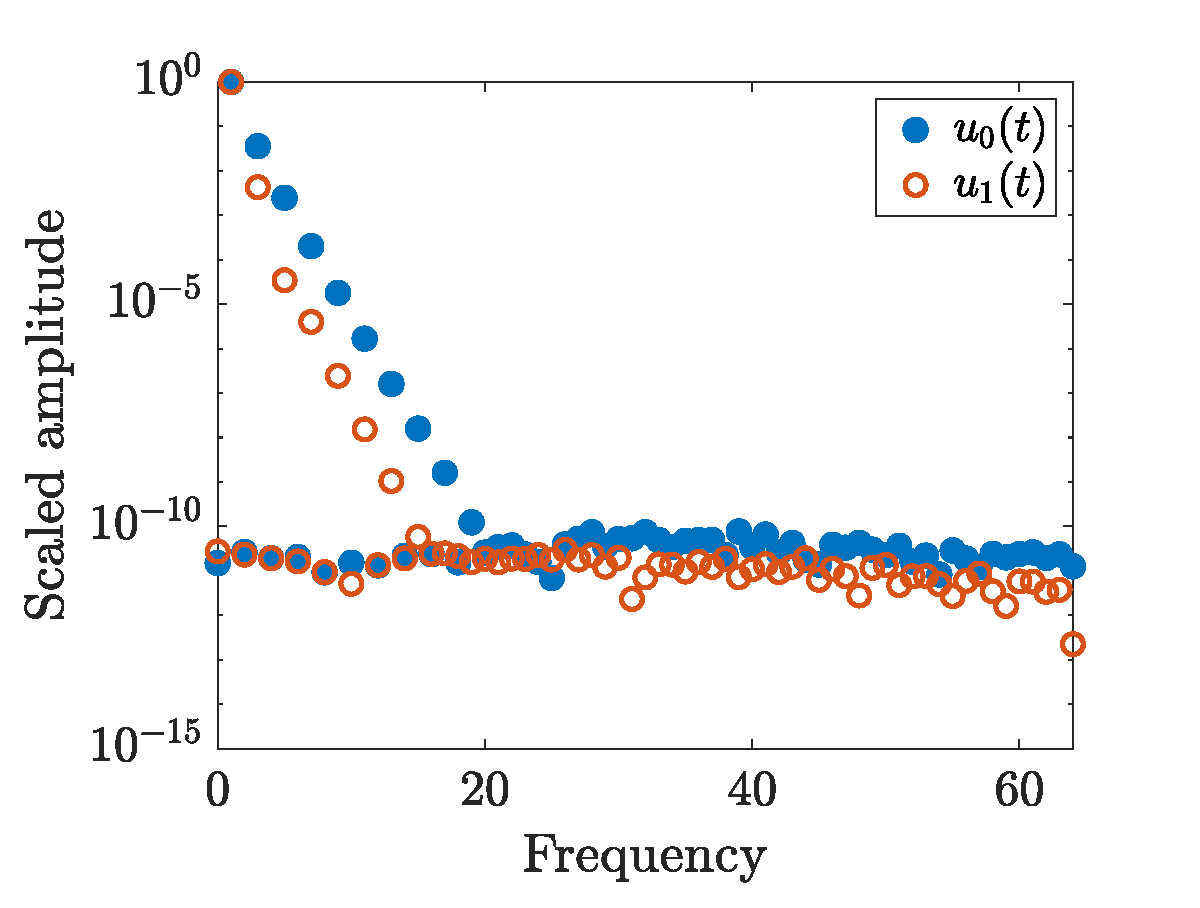
\includegraphics[width=8cm]{freqdecay.eps} 
	\end{center}
	\caption{Semilog plot showing decay of Fourier frequencies for single-site breather with $d=0.25$ at center site $u_0(t)$ and adjacent site $u_1(t)$. Vertical axis is rescaled so that fundamental frequency has amplitude of 1.}
	\label{fig:freqdecay}
\end{figure}

\cref{fig:double} shows the initial conditions (solution at $t=0$) for the out-of-phase (top) and in-phase (bottom) double breather at $d = 0.25$, together with their Floquet spectra and the eigenfunction corresponding to the interaction Floquet eigenmode. The out-of-phase double breather has a pair of interaction Floquet eigenmodes on the unit circle, while the in-phase double breather has a pair of real interaction Floquet eigenmodes. We note that the solvability condition $M < 0$ for the sine-Gordon potential.
\cref{fig:eigerror} shows the relative error in the computation of these Floquet eigenmodes, using the formula \cref{eq:inteigsdouble}. As expected, the relative error increases with the coupling parameter $d$, and decreases with the separation distance $N$. \cref{fig:SGintersite} shows the initial condition $u_n(0)$ and Floquet spectra for two special two-site breathers, for which the two excited sites at the AC limit are in adjacent lattice nodes. We will call these adjacent breathers.
As predicted by \cite{cuevas-maraver2016}, the in-phase adjacent breather is unstable, and the out-of-phase adjacent breather is spectrally stable, at least for small $d$. The two copies of the primary breather in the adjacent breather are not well separated, thus the eigenvalue results do not apply.

\begin{figure}
	\begin{center}
	\begin{subfigure}{0.3\linewidth}
		\caption{}
		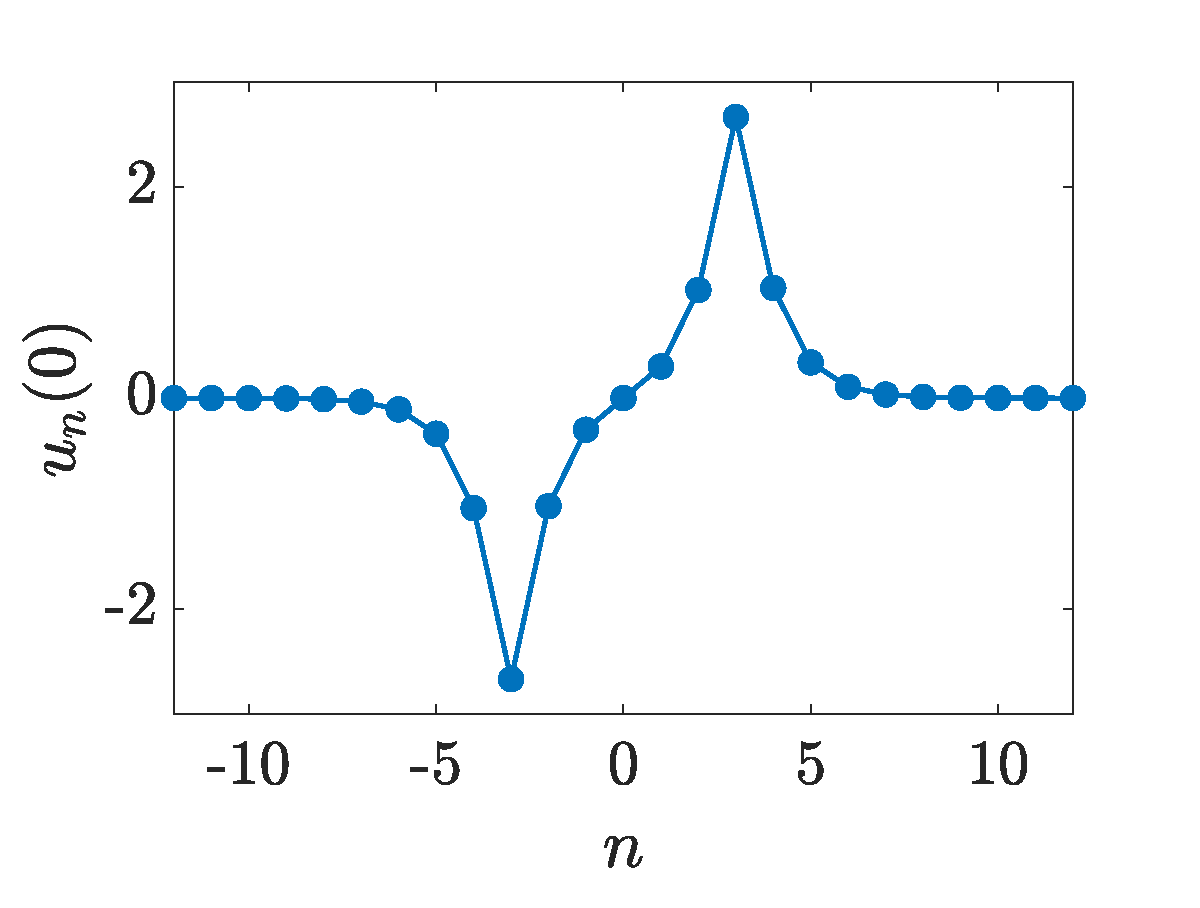
\includegraphics[width=5.5cm]{doubleun0.eps} \hspace{-0.5cm}
		\label{fig:doublea}
	\end{subfigure}
	\begin{subfigure}{0.3\linewidth}
		\caption{}
		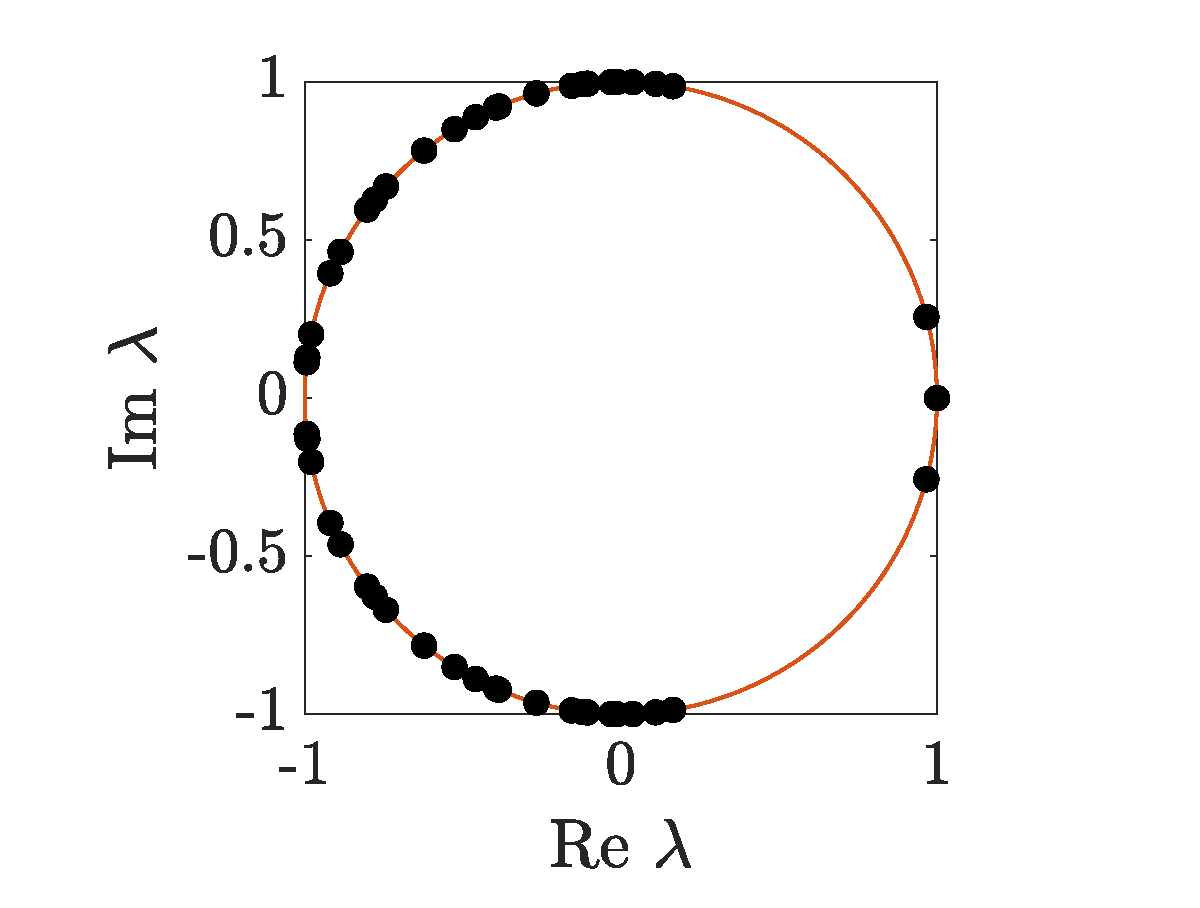
\includegraphics[width=5.5cm]{doublespec.eps} \hspace{-0.5cm}
		\label{fig:doubleb}
	\end{subfigure}
	\begin{subfigure}{0.3\linewidth}
		\caption{}
		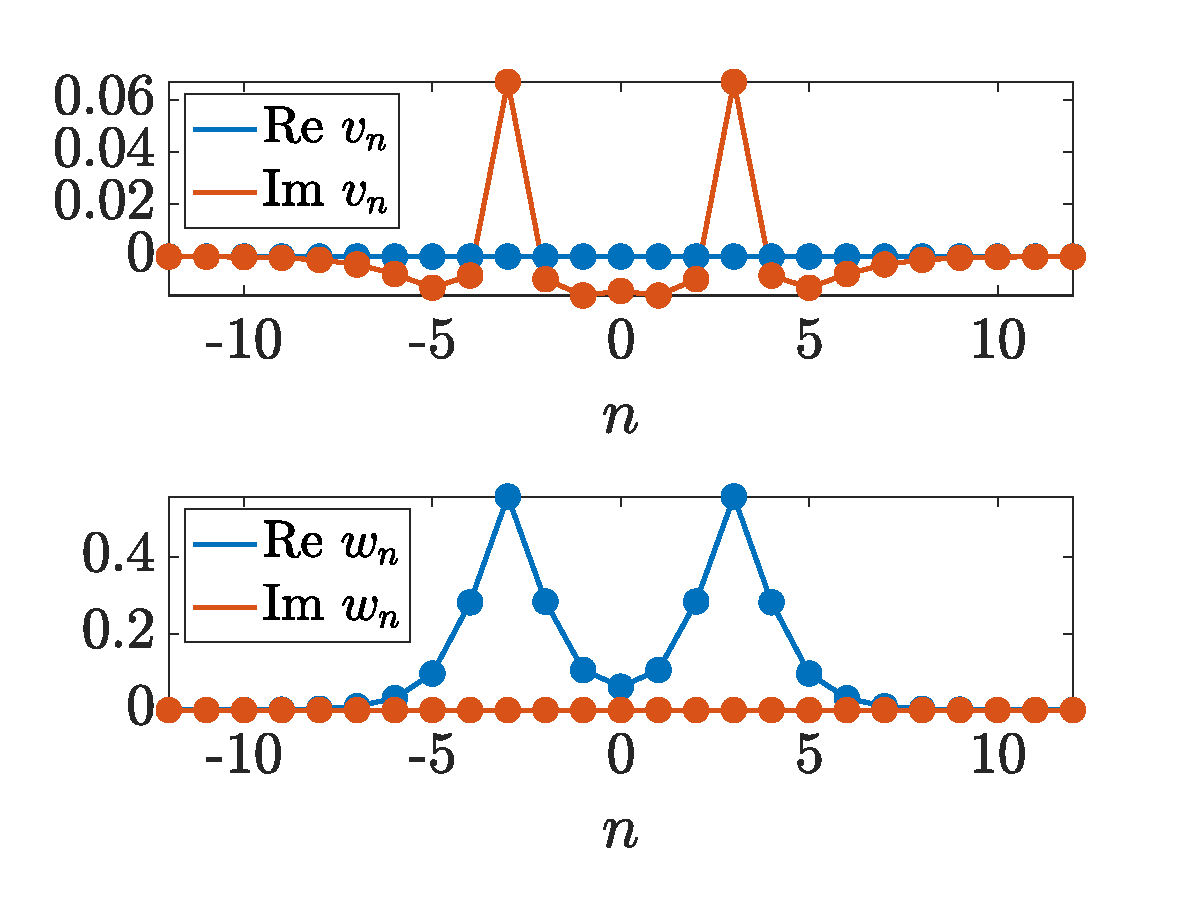
\includegraphics[width=5.5cm]{doubleinteig.eps} 
		\label{fig:doublec}
	\end{subfigure}
	\begin{subfigure}{0.3\linewidth}
		\caption{}
		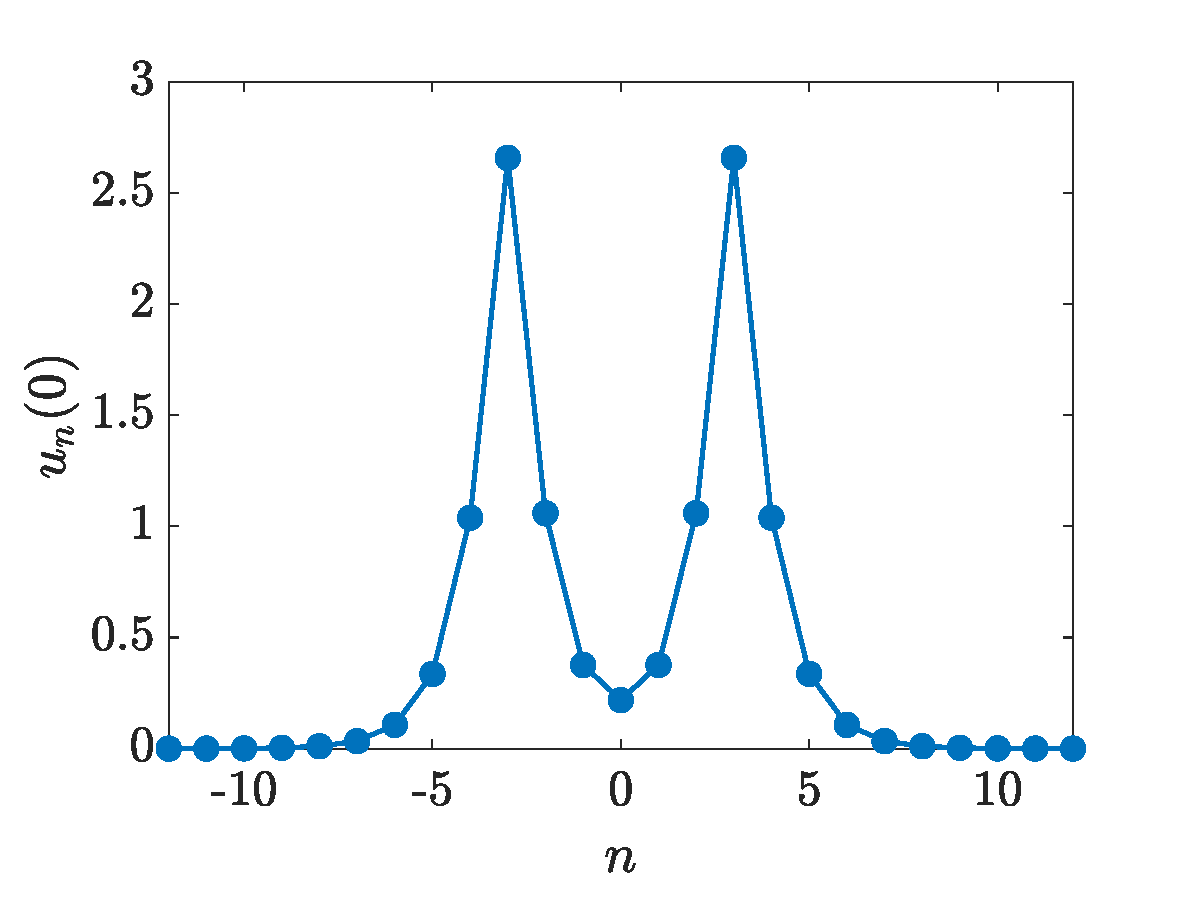
\includegraphics[width=5.5cm]{doubleppun0.eps} \hspace{-0.5cm}
		\label{fig:doubled}
	\end{subfigure}
	\begin{subfigure}{0.3\linewidth}
		\caption{}
		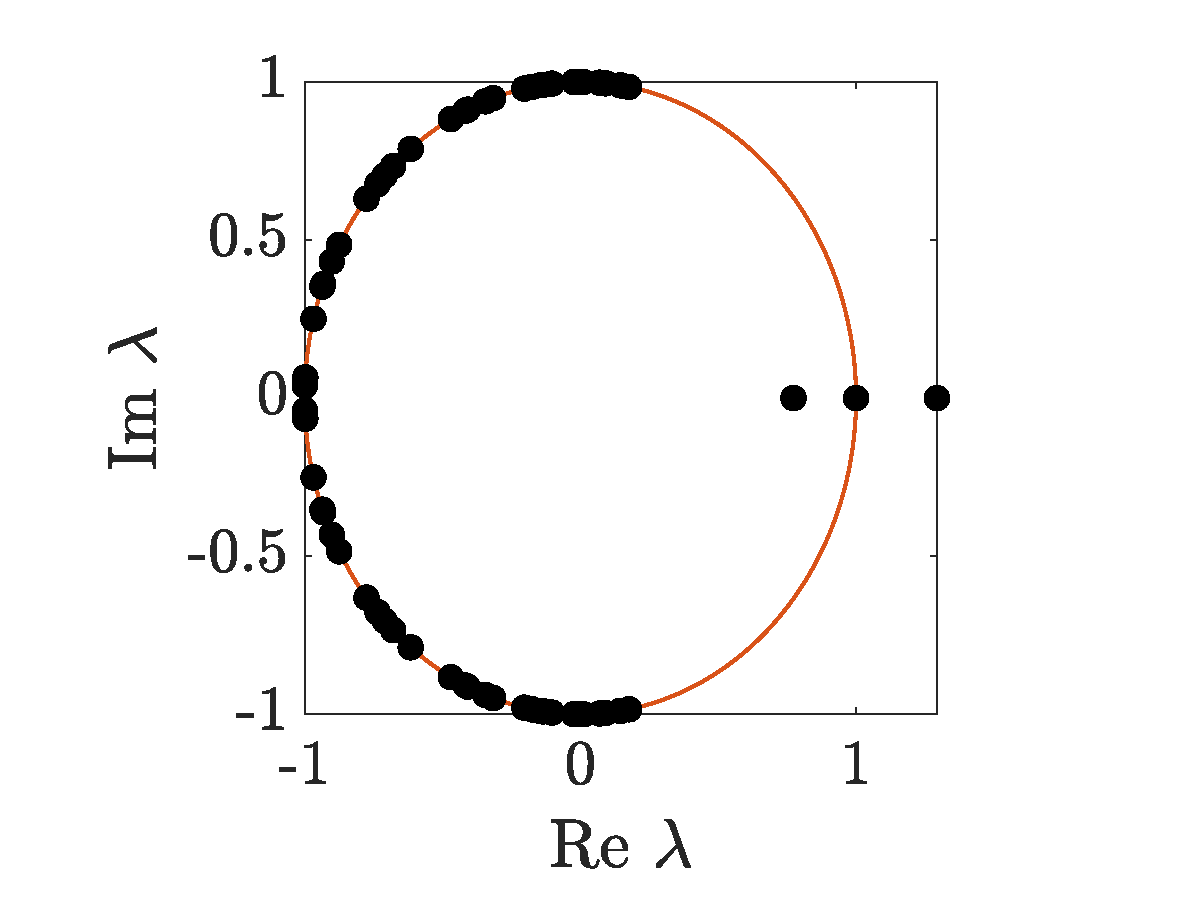
\includegraphics[width=5.5cm]{doubleppspec.eps} \hspace{-0.5cm}
		\label{fig:doublee}
	\end{subfigure}
	\begin{subfigure}{0.3\linewidth}
		\caption{}
		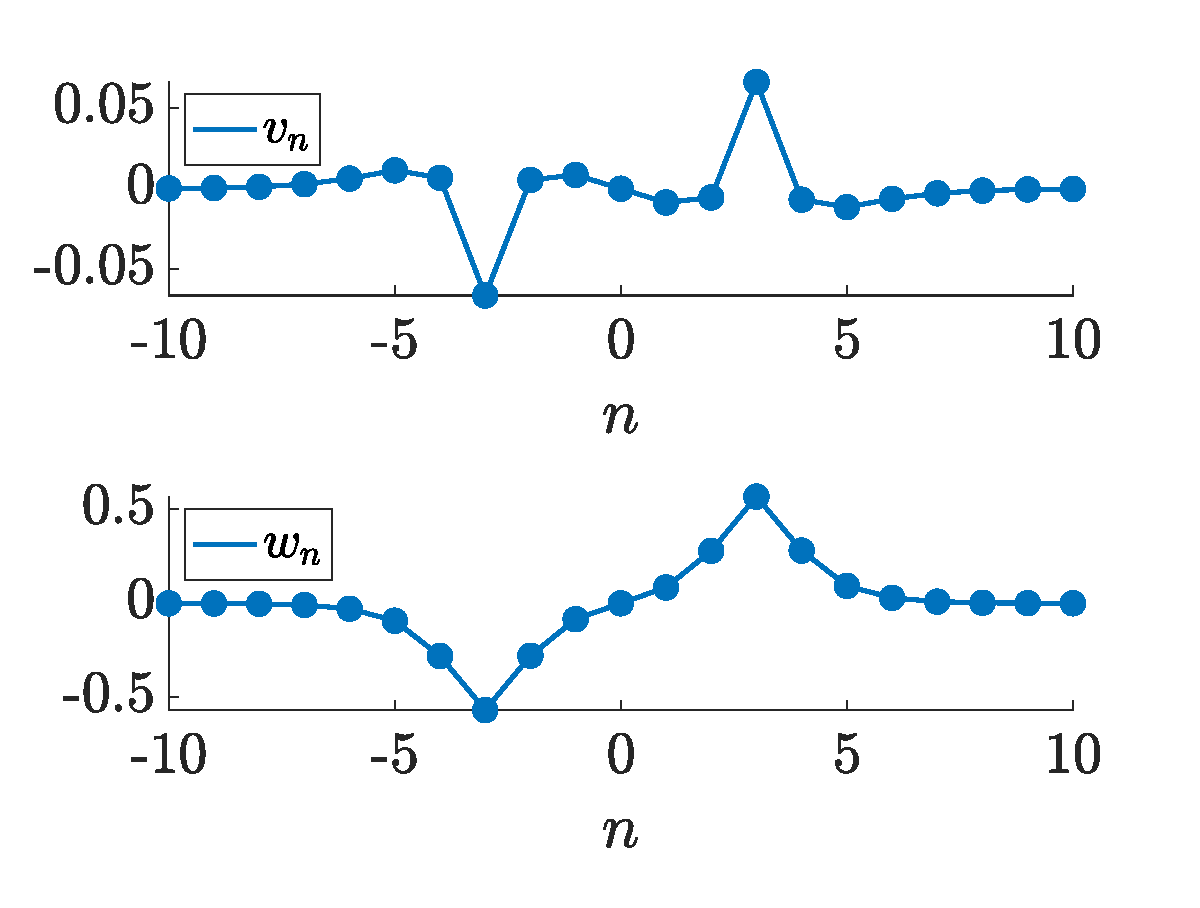
\includegraphics[width=5.5cm]{doubleppinteig.eps}
		\label{fig:doublef} 
	\end{subfigure}
	\end{center}
	\caption{Initial condition $u_n(0)$, Floquet spectrum, and eigenfunction corresponding to interaction eigenvalue for out-of-phase double breather (top) and in-phase double breather (bottom). Coupling parameter $d = 0.25$, breather distance $N_1 = 6$.}
	\label{fig:double}
\end{figure}

\begin{figure}
	\begin{center}
	\begin{subfigure}{0.3\linewidth}
		\caption{}
		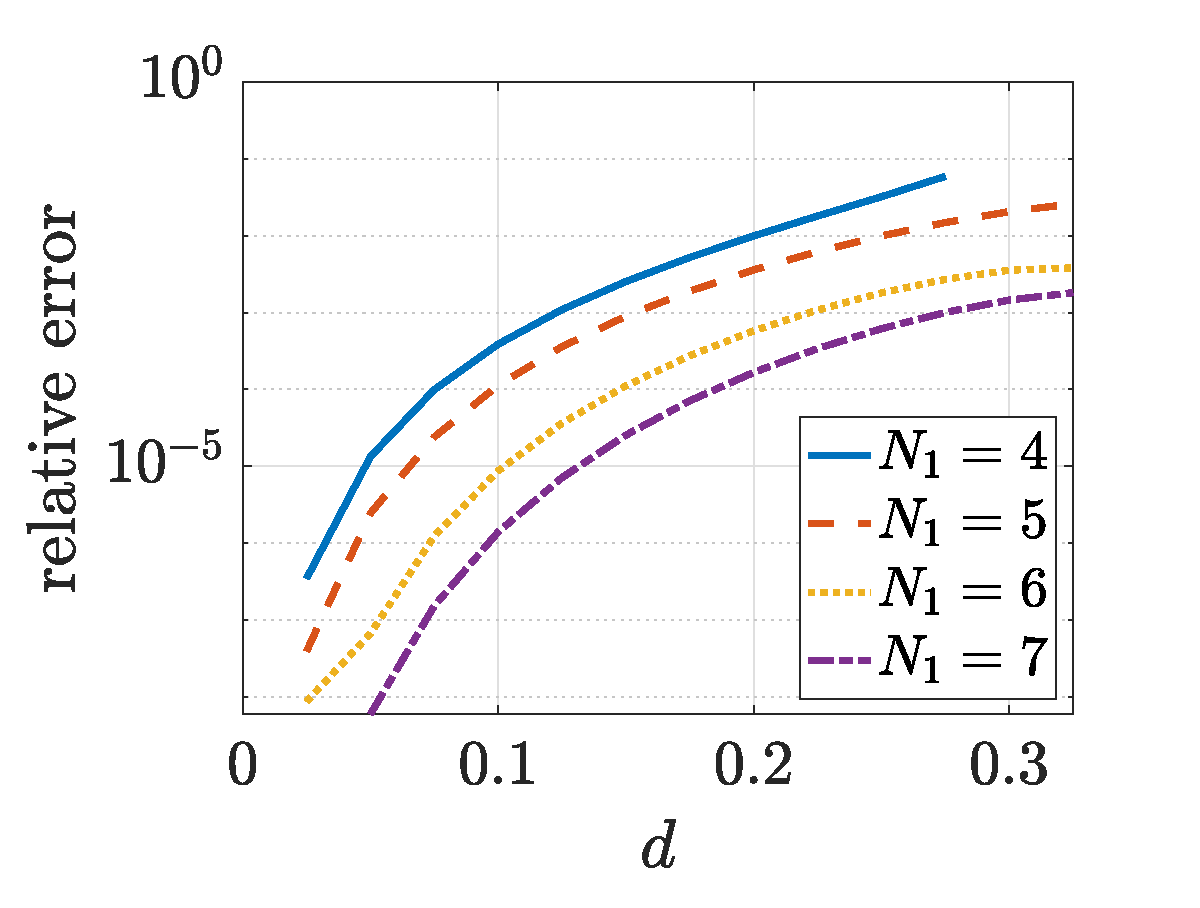
\includegraphics[width=5.5cm]{doubleeigerrord.eps} \hspace{-0.5cm}
		\label{fig:eigerrora} 
	\end{subfigure}
	\begin{subfigure}{0.3\linewidth}
		\caption{}
		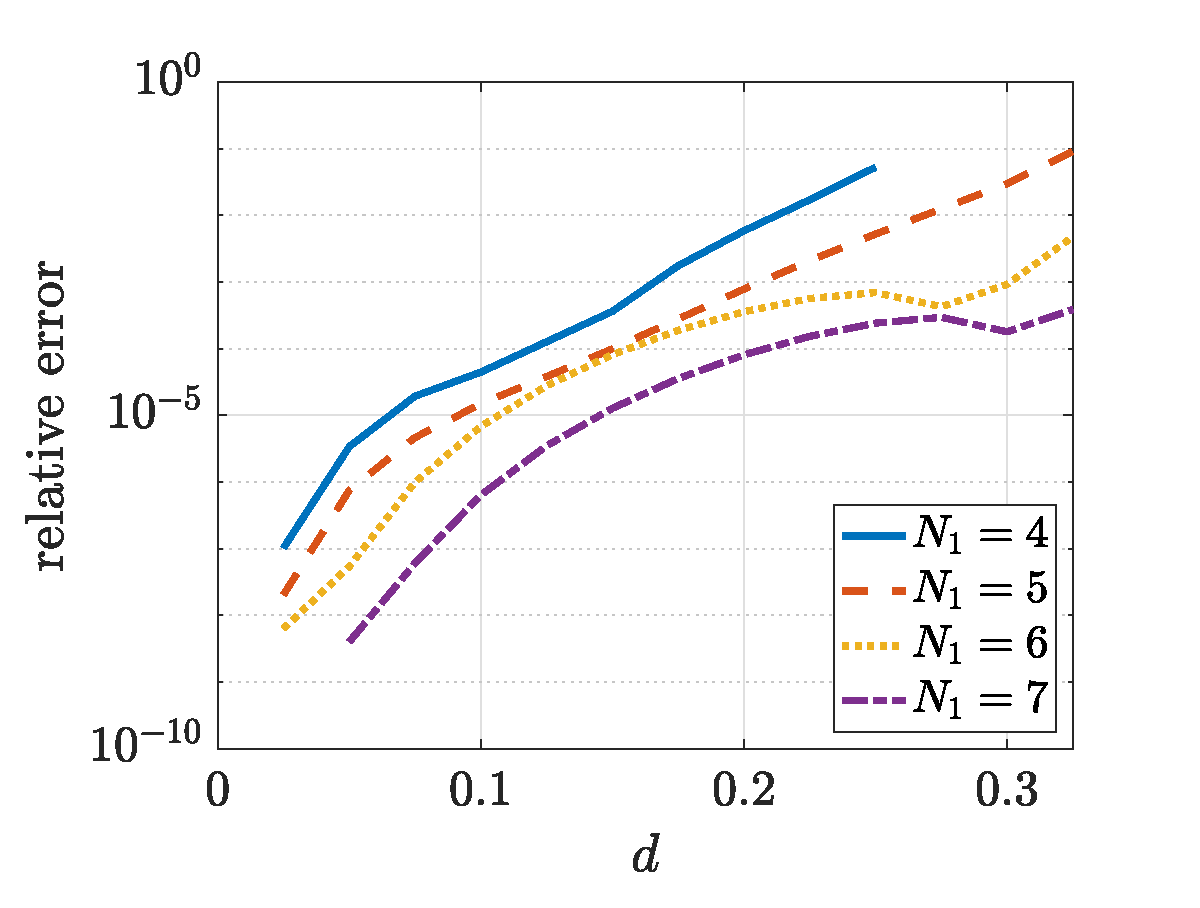
\includegraphics[width=5.5cm]{doubleppeigerrord.eps} \hspace{-0.5cm}
		\label{fig:eigerrorb} 
	\end{subfigure}
	\begin{subfigure}{0.3\linewidth}
		\caption{}
		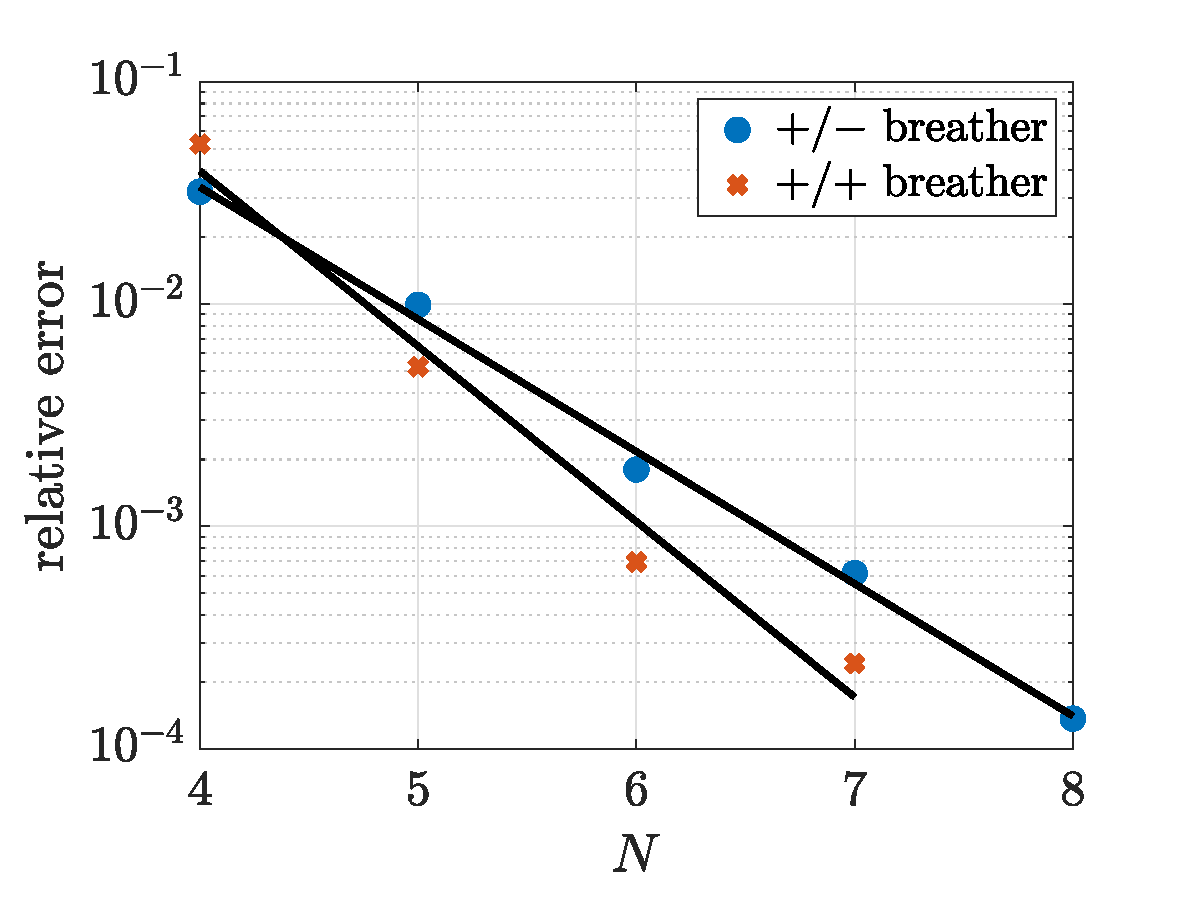
\includegraphics[width=5.5cm]{doubleeigerrorN.eps} 
		\label{fig:eigerrorc} 
	\end{subfigure}
	\end{center}
	\caption{Semilog plot of relative error of interaction eigenvalue computation vs. $d$ for out-of-phase double breathers (a) and in-phase double breathers (b) for breather distance $N_1 = 4,5,6,7$. (c) Semilog plot of relative error of double breathers vs. $N$ for coupling parameter $d = 0.25$.}
	\label{fig:eigerror}
\end{figure}

\begin{figure}
	\begin{center}
	\begin{subfigure}{0.3\linewidth}
		\caption{}
		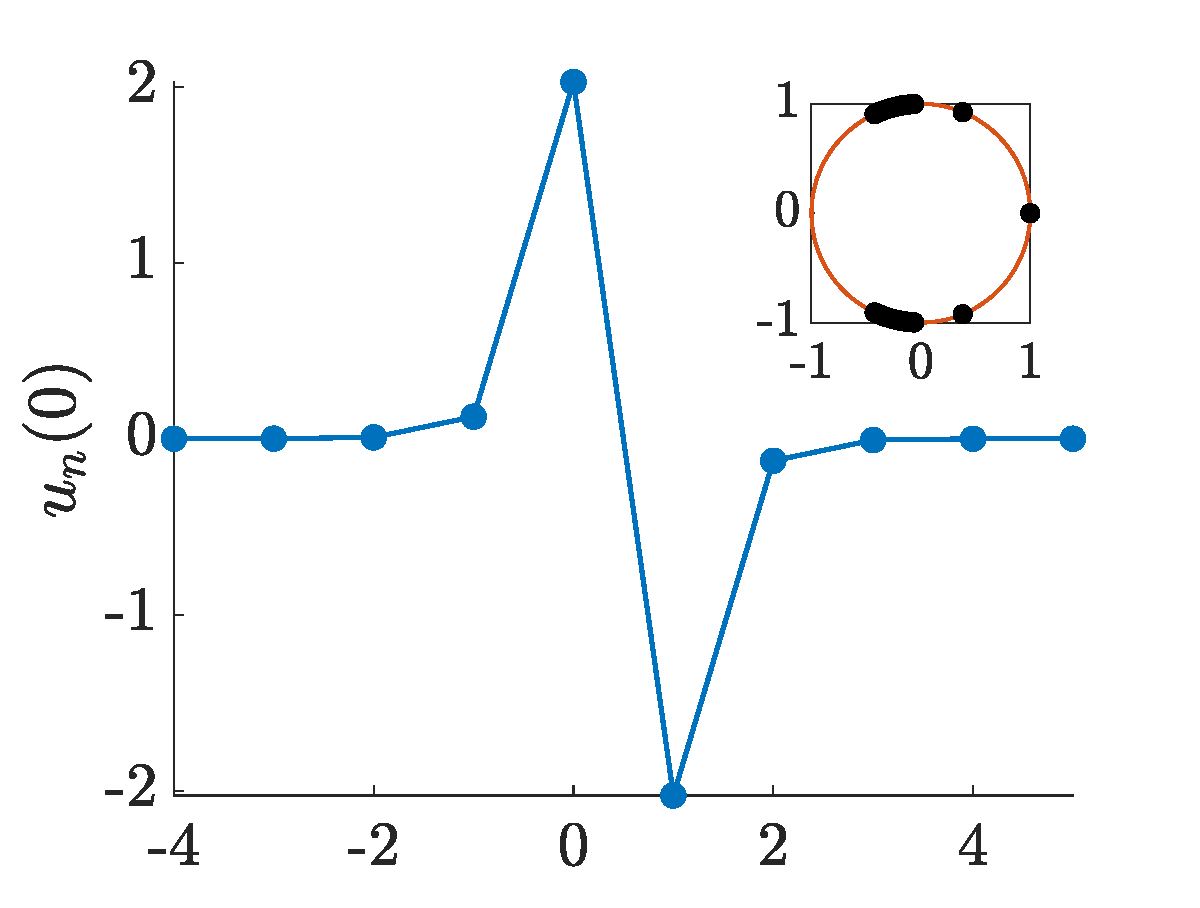
\includegraphics[width=5.5cm]{SGintersitepm.eps} \hspace{-0.5cm}
		\label{fig:SGintersitea} 
	\end{subfigure}
	\begin{subfigure}{0.3\linewidth}
		\caption{}
		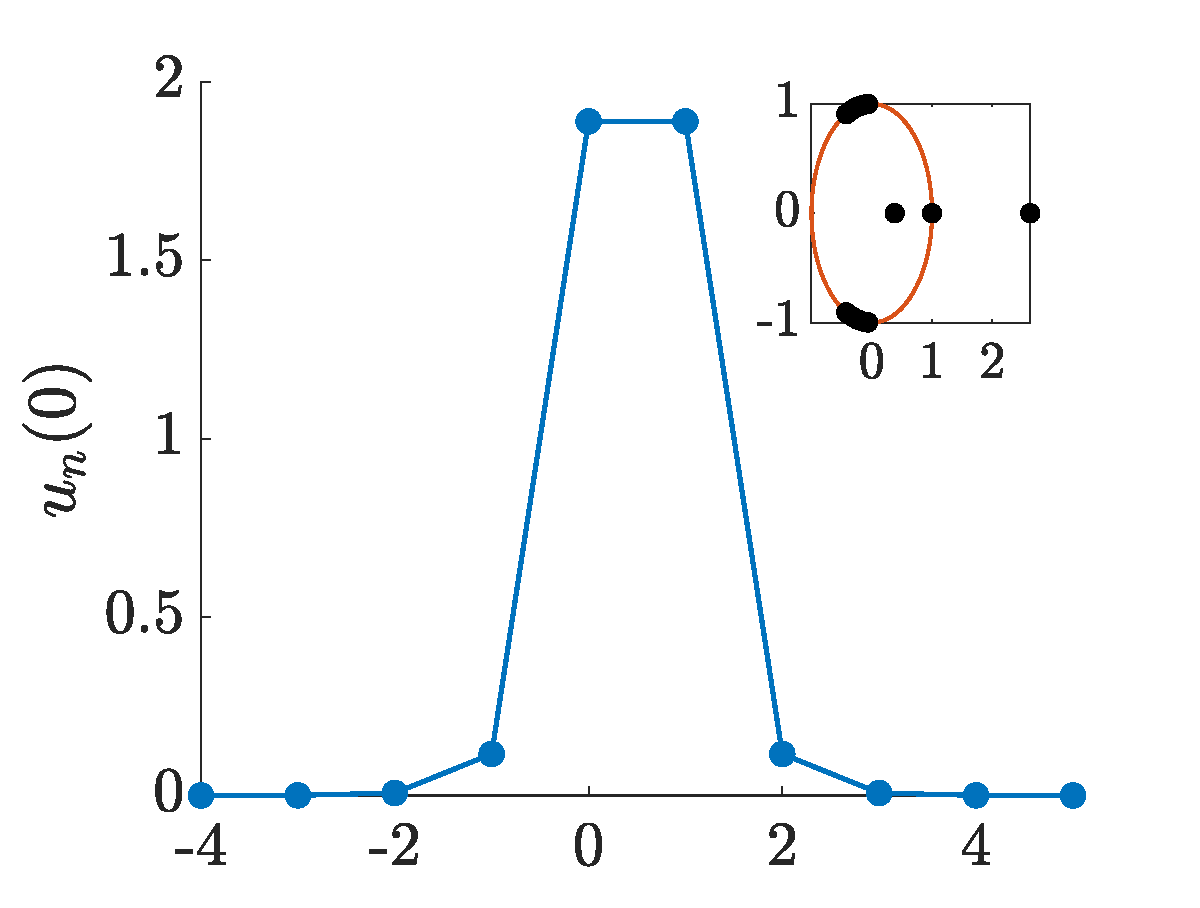
\includegraphics[width=5.5cm]{SGintersitepp.eps} \hspace{-0.5cm}
		\label{fig:SGintersiteb} 
	\end{subfigure}
	\end{center}
	\caption{Initial condition $u_n(0)$ and Floquet spectrum (inset) for in-phase adjacent breather (a), and out-of-phase adjacent breather (b). Coupling parameter $d=0.1$. }
	\label{fig:SGintersite}
\end{figure}

\cref{fig:bifdiagSGoop1} shows the bifurcation diagram for an out-of-phase double breather, starting from the AC limit. The parameter continuation starts on the lower branch, where the double breather has a pair of interaction multipliers on the unit circle (a). The upper branch is a double breather comprising two in-phase adjacent breathers (j), which we recall are unstable; this breather has two pairs of real interaction multipliers. The middle branch is an asymmetric double breather, comprising one single-site breather and one in-phase adjacent breather (k); this breather has one pair of real interaction multipliers, and one pair of interaction multipliers on the unit circle. There is a corresponding branch (not shown) where the order of the two breathers is reversed. As $d$ is increased along the lower branch, a pair of internal modes appears on the unit circle (b); these have opposite Krein signature from the nearby interaction Floquet mode. These collide and move off of the unit circle (c-d). At this point, a second pair of internal modes has appeared on the unit circle, which then passes between the first pair of Floquet modes (e). The Floquet modes that collided recombine near point (f), which is located most of the way to the first bifurcation point. Between (g) and (h), the second pair of internal modes collides at (1,0) and moves off of the unit circle. Between (i) and (j), there is a pitchfork bifurcation which produces the middle branches of the bifurcation diagram; at this point, the first pair of internal modes collides and moves off of the unit circle.

\begin{figure}
	\hbox{
	\hspace{-2cm}
	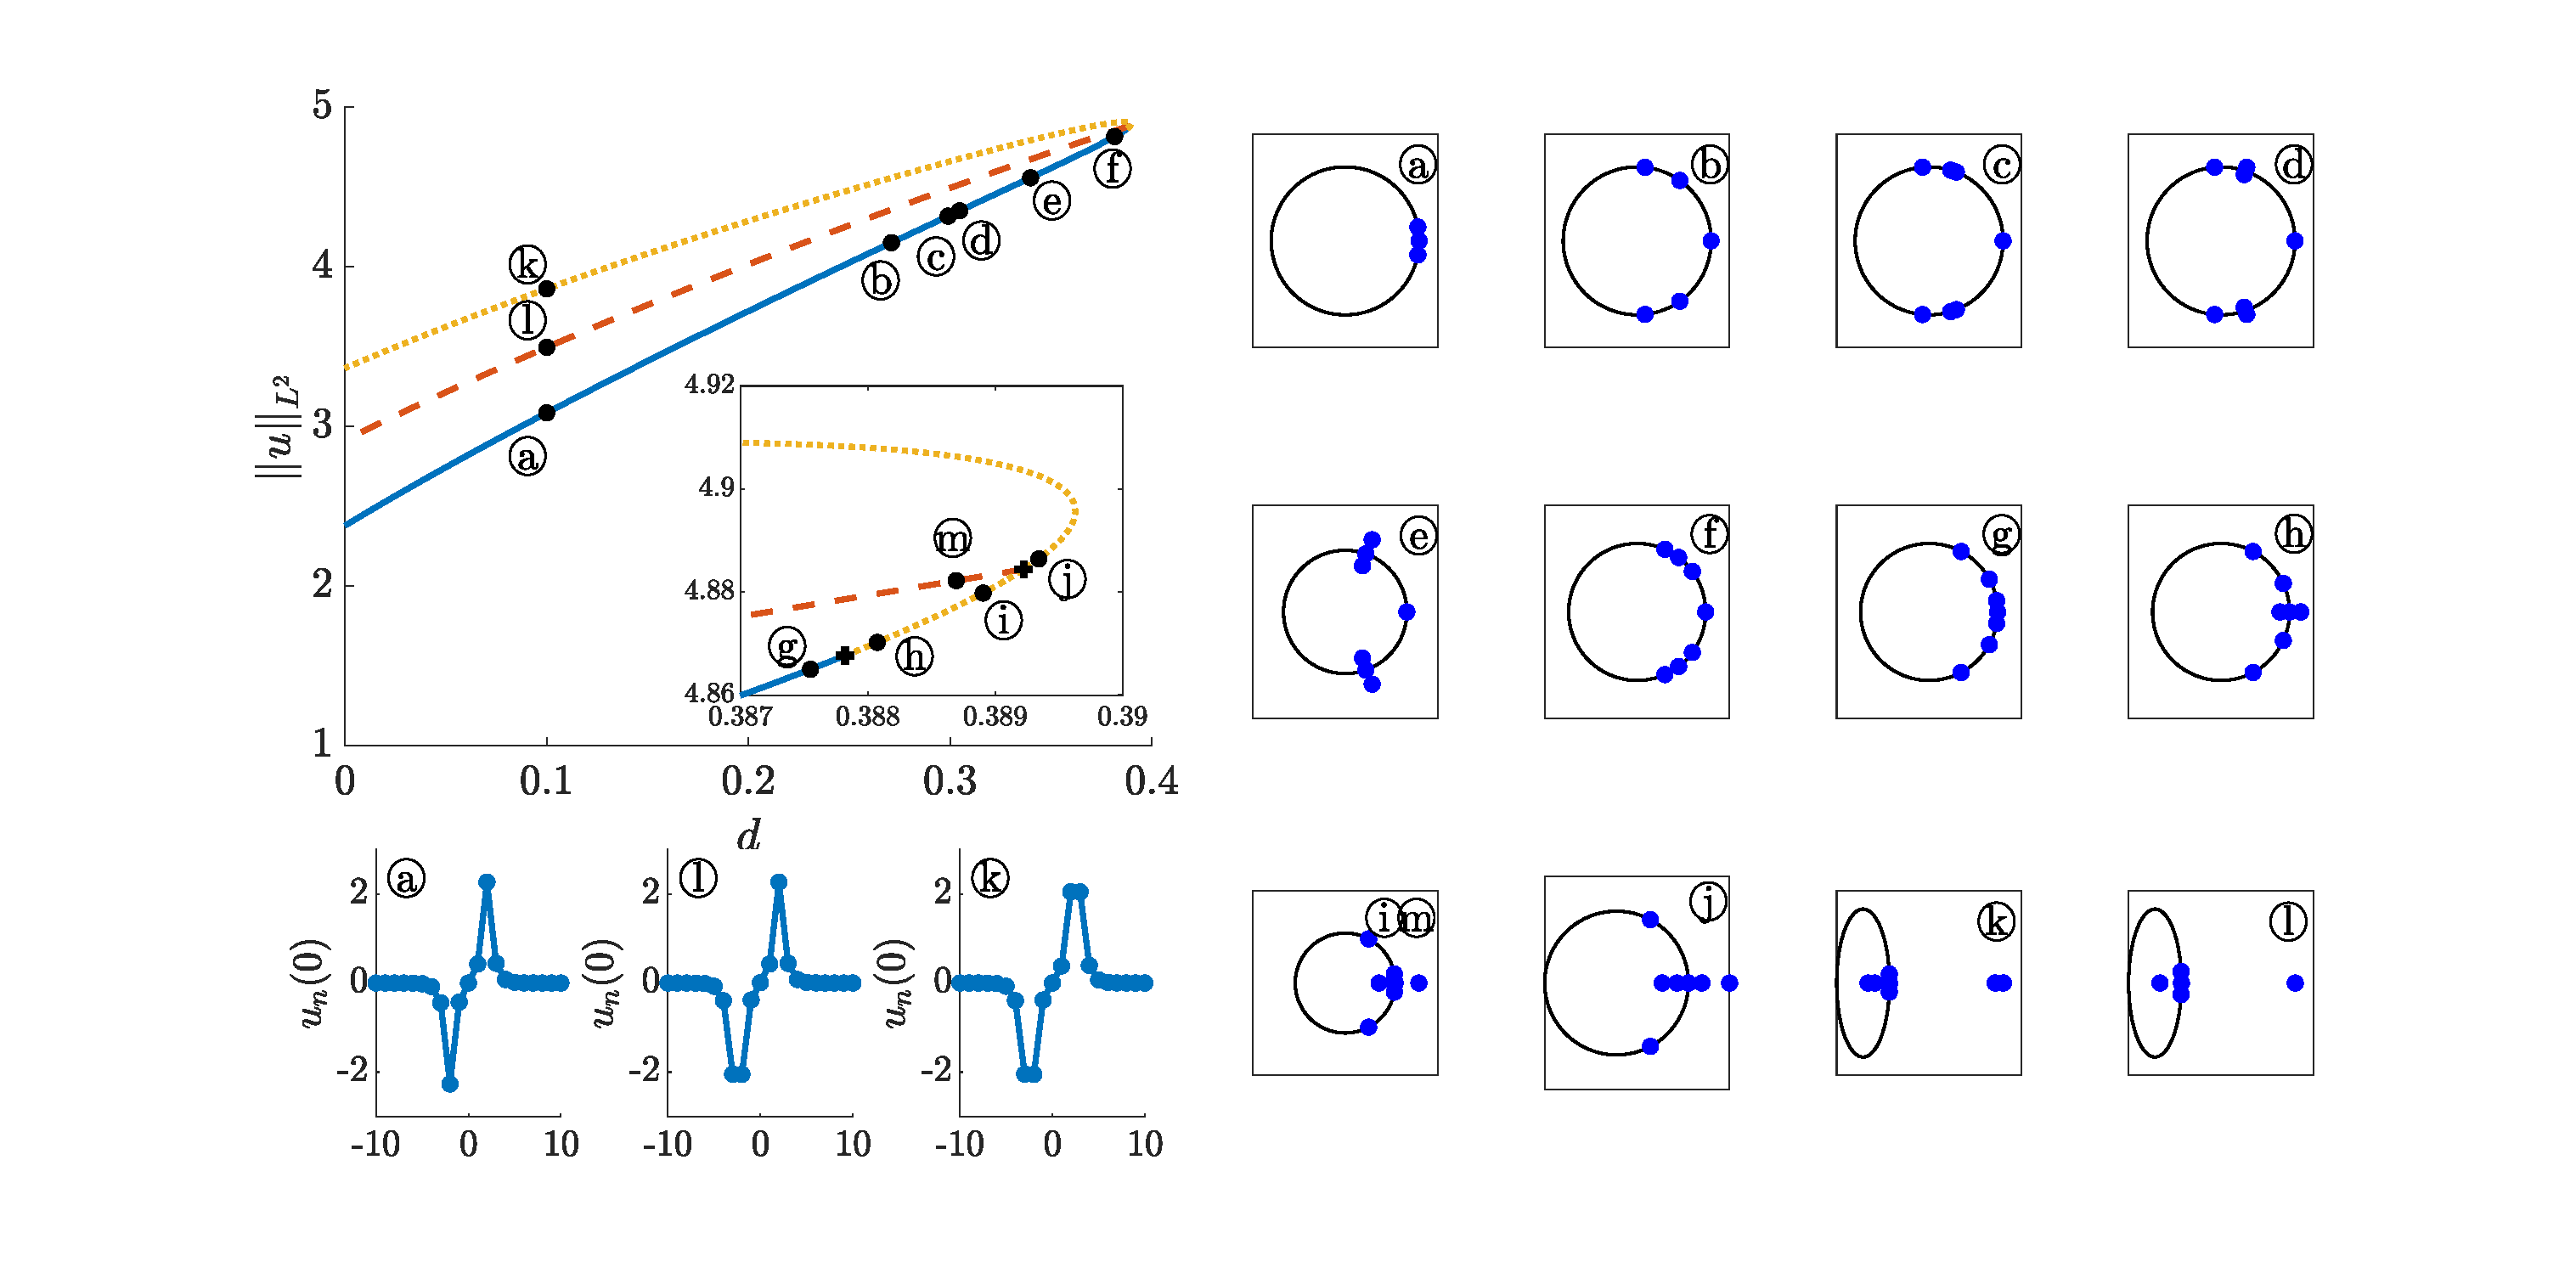
\includegraphics[width=20cm]{bifdiagSGoppositeN4.eps} 
	}
	\caption{Bifurcation diagram for out-of-phase double breather with $N_1 = 4$. Points of interest are marked with black dots and labeled with circled letters, which correspond to Floquet spectra. Continuous spectrum bands are not shown for clarity. Bifurcations are indicated with a black cross.}
	\label{fig:bifdiagSGoop1}
\end{figure}

\cref{fig:bifdiagSGip1} shows the bifurcation diagram for an in-phase double breather, again starting from the AC limit. The diagram is qualitatively similar, in that the two bifurcations result from collisions of internal modes at (1,0). The main difference is that since the starting in-phase breather has a pair of real interaction Floquet eigenmodes, these are not involved with any collisions with internal modes. In both cases, there is a turning point in the bifurcation diagram at a critical value $d_0$ of the coupling parameter $d$, at which point the parameter continuation reverses direction in $d$. For the out-of-phase double breather, this occurs after both bifurcations (see inset in \cref{fig:bifdiagSGoop1}), whereas for the in-phase double breather, this occurs between the two bifurcation points (see inset in \cref{fig:bifdiagSGip1}). A plot of the turning point $d_0$ vs. the separation distance $N$ in \cref{fig:bifdiagSGip1} suggests that $d_0$ increases linearly with $N$.

\begin{figure}
	\hbox{
	\hspace{-2cm}
	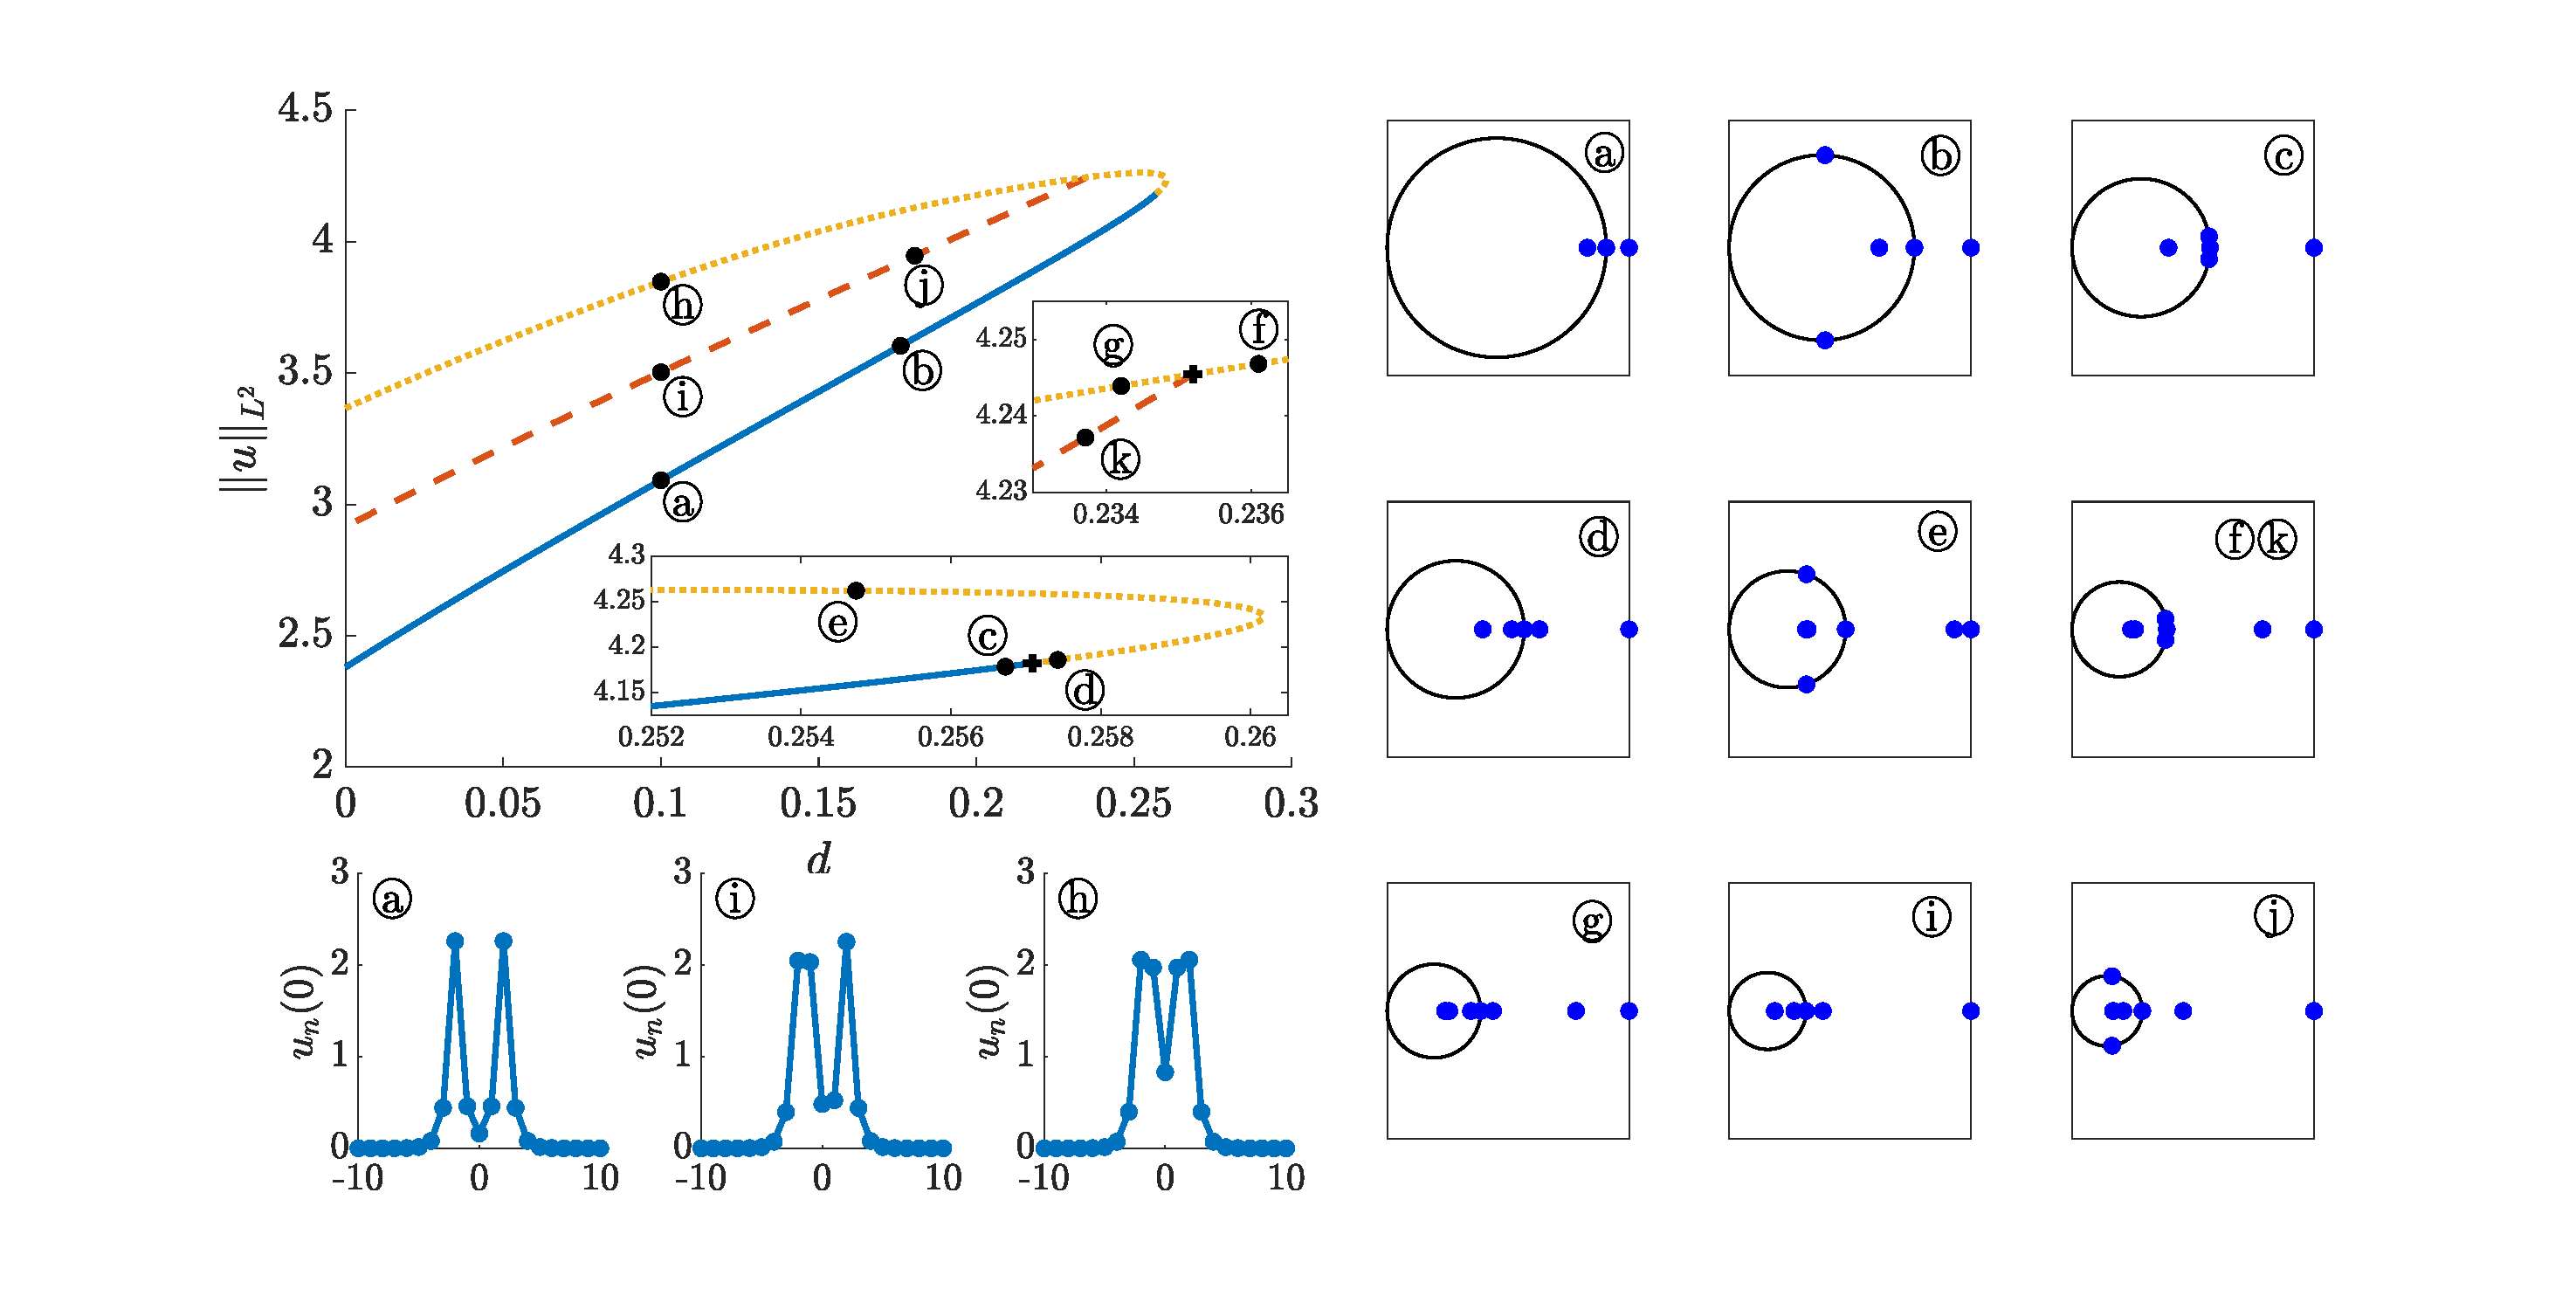
\includegraphics[width=20cm]{bifdiagSGinphaseN4.eps} 
	}
	\caption{Bifurcation diagram for in-phase double breather with $N_1 = 4$. Points of interest are marked with black dots and labeled with circled letters, which correspond to Floquet spectra. Continuous spectrum bands are not shown for clarity. Bifurcations are indicated with a black cross. }
	\label{fig:bifdiagSGip1}
\end{figure}

\begin{figure}
	\begin{center}
	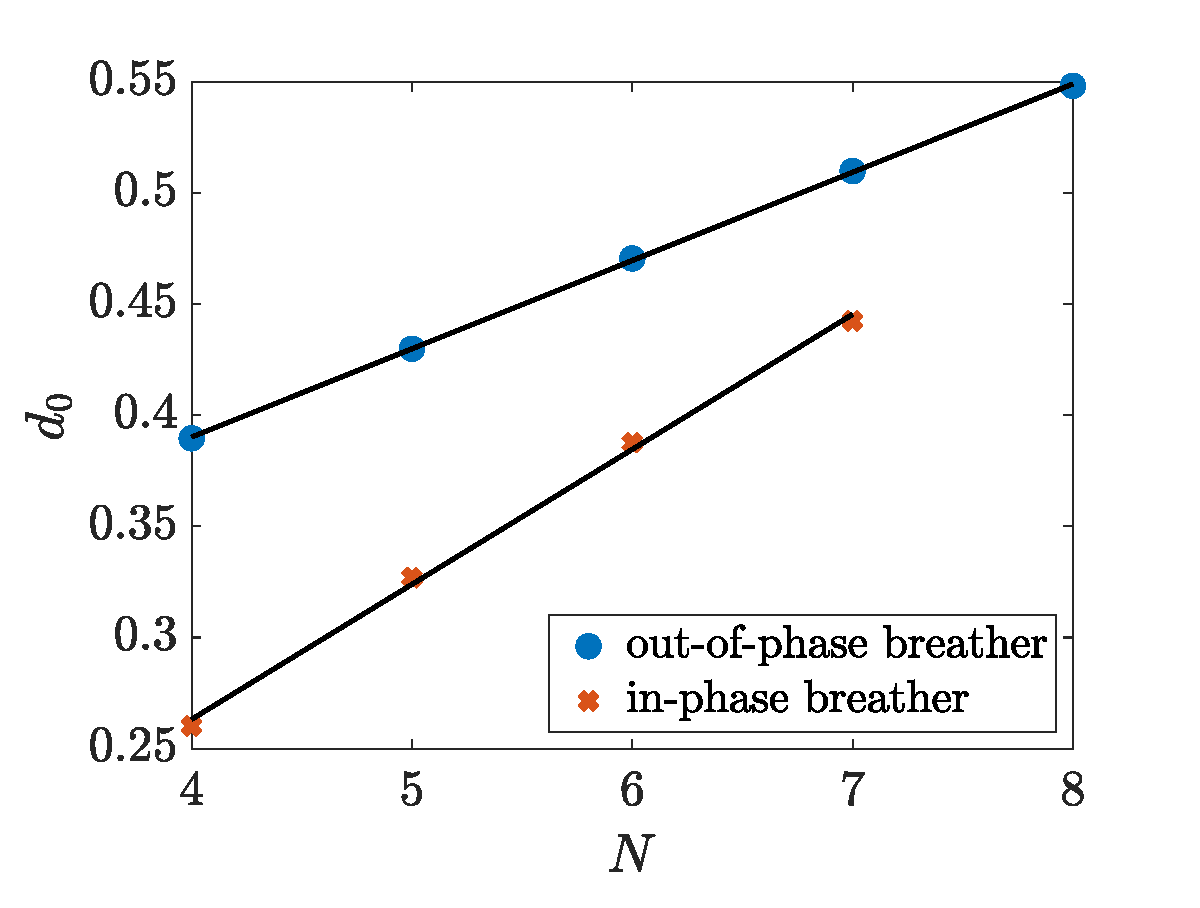
\includegraphics[width=8cm]{doubled0vsN.eps} 
	\end{center}
	\caption{Turning point of parameter continuation $d_0$ vs separation distance $N$ for out-of-phase and in-phase double breathers.}
	\label{fig:SGd0}
\end{figure}

Finally, we demonstrate the effect of the interaction eigenmodes on the dynamics of the double breathers by performing timestepping experiments. For a timestepping scheme, we use a symplectic and symmetric implicit Runge-Kutta method \cite{HairerBook} to preserve the symplectic structure of the Hamiltonian system. Specifically, we use the MATLAB implementation of the \texttt{irk2} scheme of order 12 from \cite{Hairer2003}.
For each experiment, we perturb the stationary breather by adding a small multiple of the eigenfunction $v_n$ corresponding to the interaction Floquet multiplier $\mu$. For a double breather $u_n(t)$, let $u_L(t) = u_{-N_1^-}(t)$ and $u_R(t) = u_{N_1^+}(t)$ be the center sites of the left and the right breather, respectively. When the out-of-phase double breather is perturbed, the peak amplitudes of $u_L(t)$ and $u_R(t)$ oscillate in opposite directions with frequency given by the imaginary part of $\log(\mu)/T$ (see top row of \cref{fig:timestepSG}), with relative error less than 0.001. When the in-phase double breather is perturbed, the oscillations in $u_L(t)$ increase in amplitude and decrease in frequency, while those in $u_R(t)$ decrease in amplitude and increase in frequency (\cref{fig:timestepSGc}). (These are reversed if the perturbation is in the opposite direction). The growth rate of the difference in $L^2$ norm between the perturbed and unperturbed solutions is given $\mu^{1/T}$, with a relative error of less than 0.001, where $\mu > 1$ is the larger of the Floquet multiplier pair.

\begin{figure}
	\begin{center}
	\begin{subfigure}{0.45\linewidth}
		\caption{}
		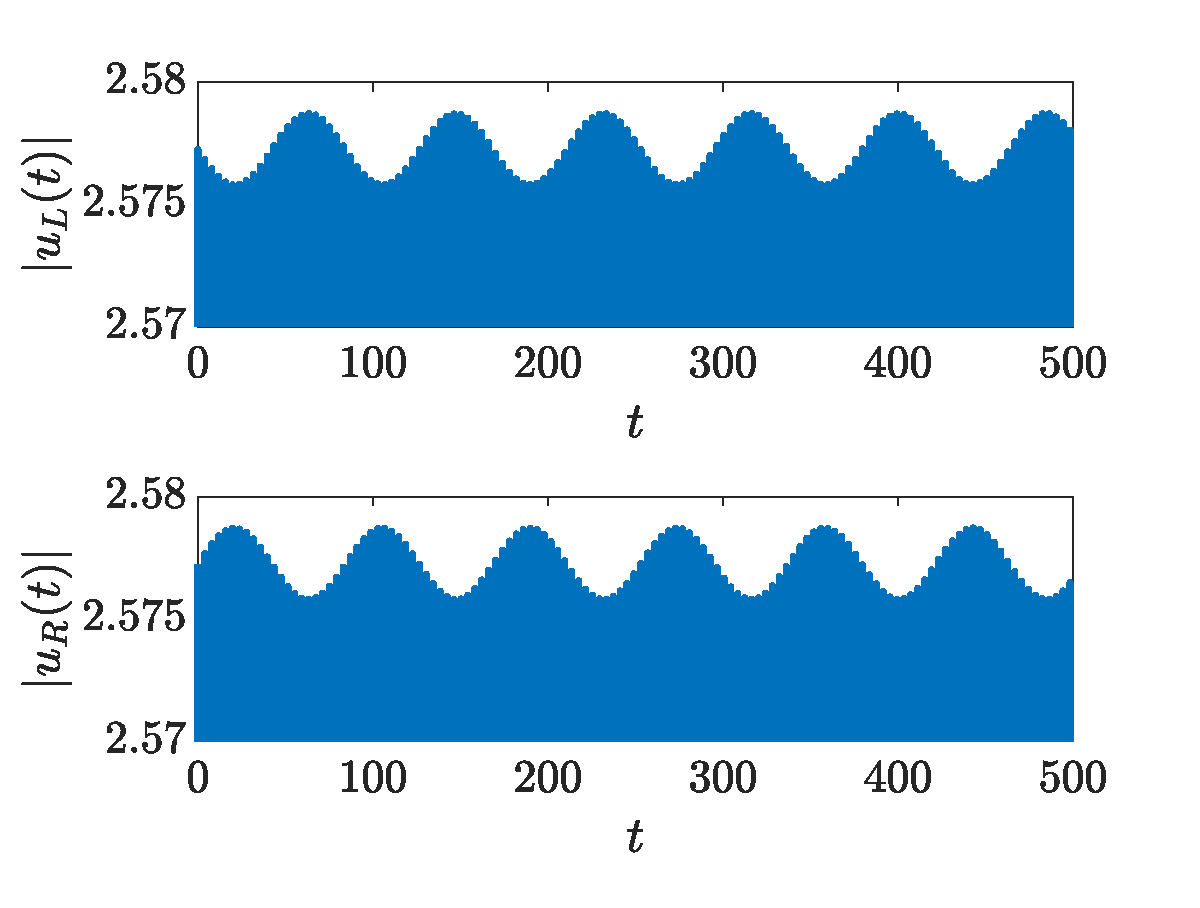
\includegraphics[width=7.5cm]{timestepN6.eps}
		\label{fig:timestepSGa}
	\end{subfigure}
	\begin{subfigure}{0.45\linewidth}
		\caption{}
		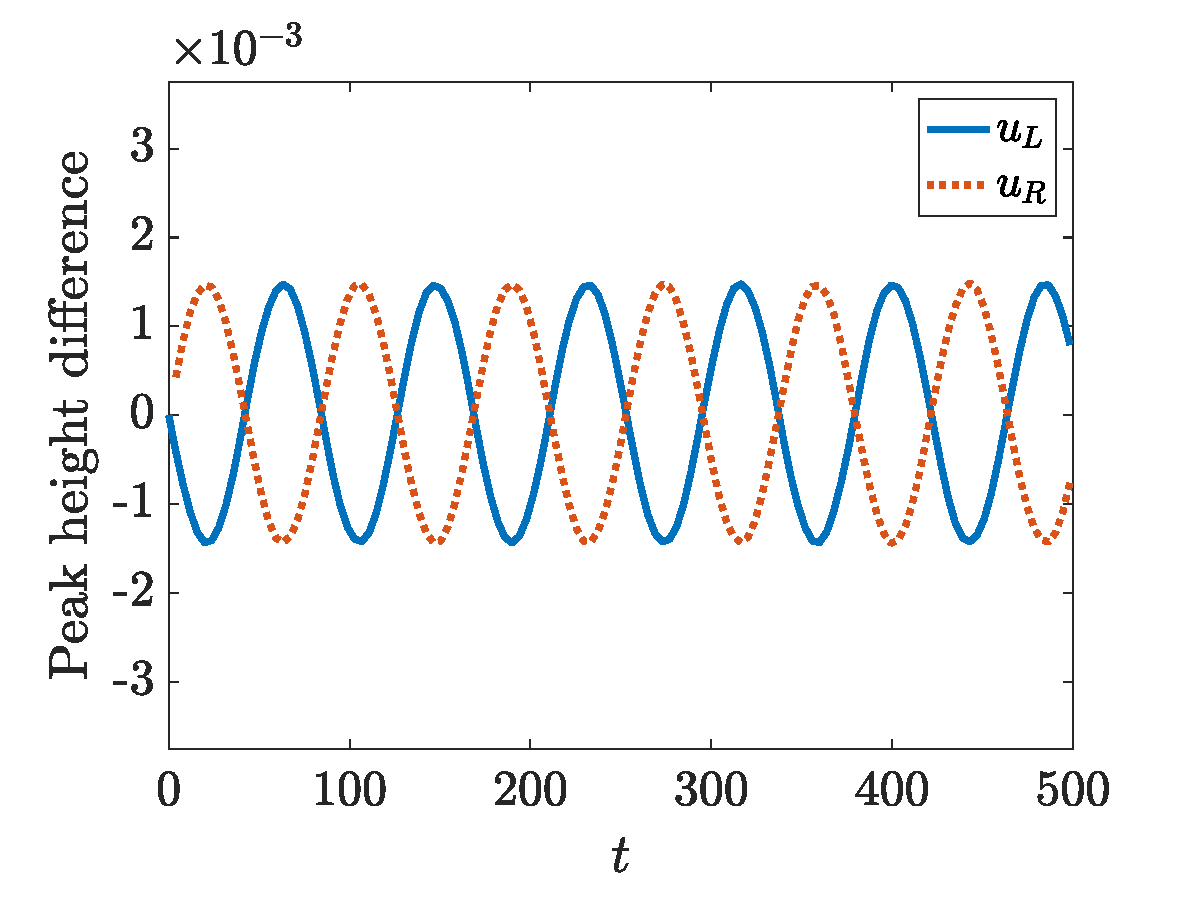
\includegraphics[width=7.5cm]{timestepN6pks.eps}
		\label{fig:timestepSGb}
	\end{subfigure}
	\begin{subfigure}{0.45\linewidth}
		\caption{}
		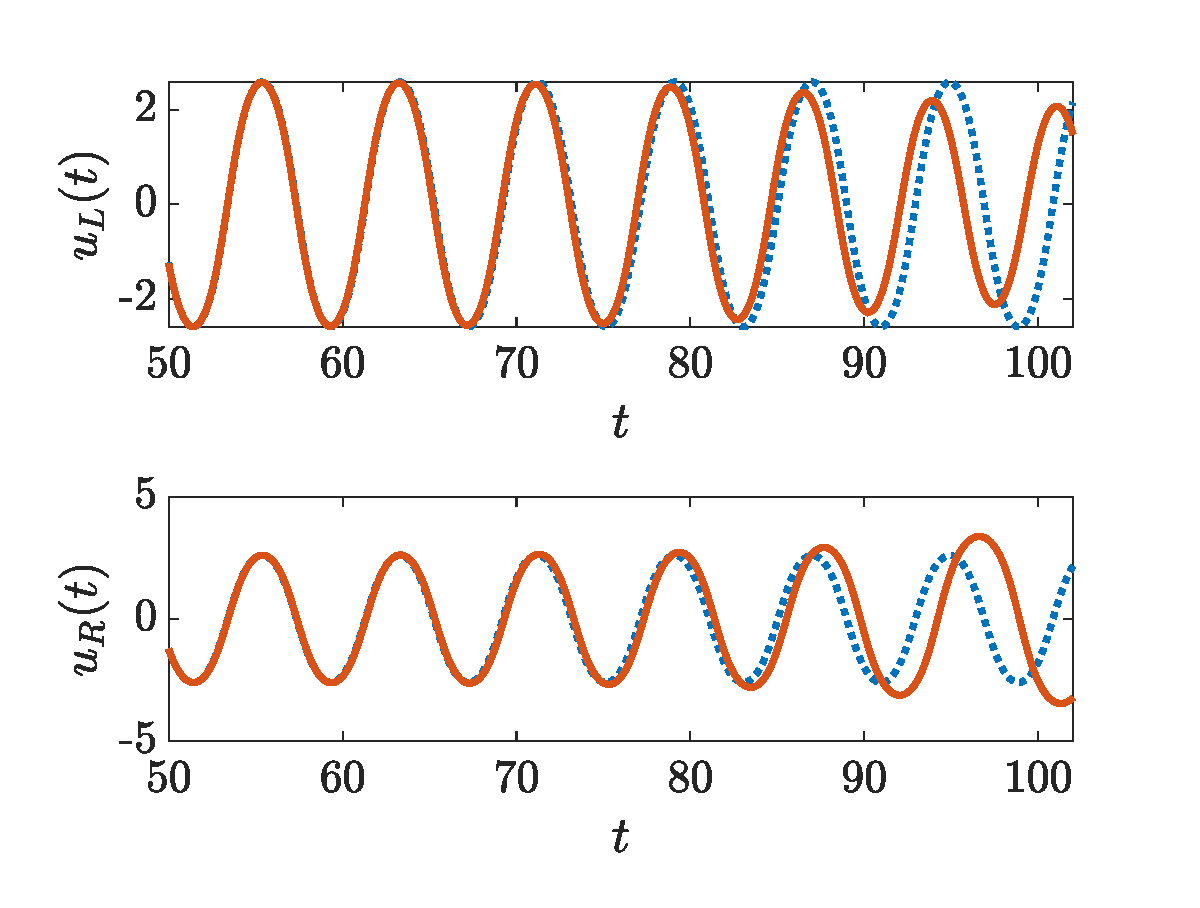
\includegraphics[width=7.5cm]{timestepN6pp.eps}
		\label{fig:timestepSGc}
	\end{subfigure}
	\begin{subfigure}{0.45\linewidth}
		\caption{}
		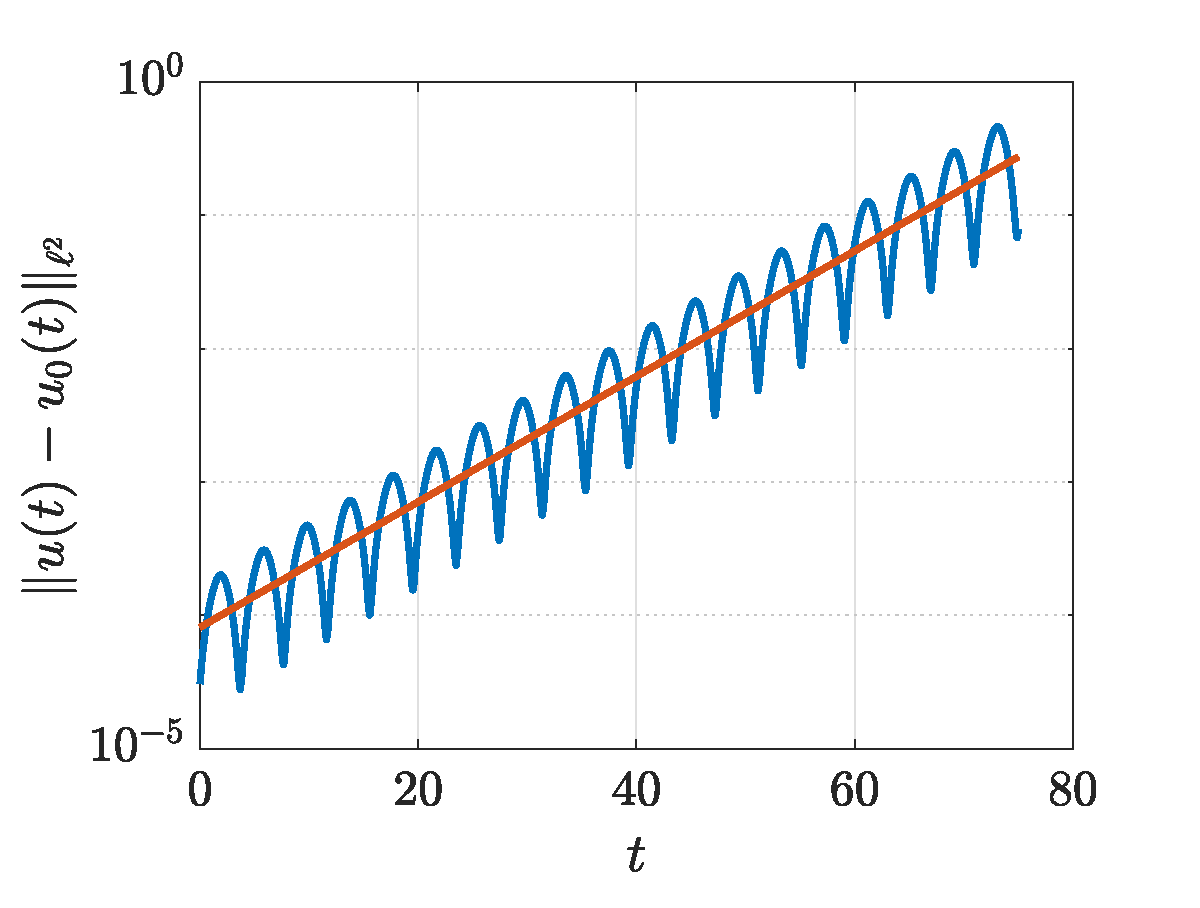
\includegraphics[width=7.5cm]{timestepN6growth.eps}
		\label{fig:timestepSGd}
	\end{subfigure}
	\end{center}
	\caption{Time evolution perturbation of out-of-phase breather (top row) and in-phase breather (bottom row). For the out-of-phase breather: (a) amplitude of the peaks of $u_L$ and $u_R$ vs. $t$, and (b) difference in this amplitude from the unperturbed breather. For the in-phase breather: (c) time evolution of $u_L$ and $u_R$ for unperturbed breather (dotted blue lines) and perturbed breather (solid orange lines), and (d) time evolution in difference of $L^2$ norm of perturbed and unperturbed breather. Coupling parameter $d=0.25$ and separation distance $N_1 = 4$ in both cases.}
	\label{fig:timestepSG}
\end{figure}

\subsection{Hard \texorpdfstring{$\phi^4$}{phi-4} potential}

The results for the soft $\phi^4$ potential are similar to those for sine-Gordon (which is expected, since the first two terms in the Taylor expansion of the sine-Gordon potential are qualitatively similar to the soft $\phi^4$ potential), thus we will not show them here. We instead look at the hard $\phi^4$ potential. \cref{fig:phi4sol} shows the initial conditions for the primary breather, the in-phase adjacent breather, and the out-of-phase adjacent breather, together with their Floquet spectra. In contrast to the sine-Gordon potential, the out-of-phase adjacent breather is unstable. The in-phase adjacent breather is spectrally stable for sufficiently small $d$ (see also Figures 4 and 6 in \cite{cuevas-maraver2016}). These agree with the results of \cites{Archilla2003,Koukouloyannis2009}. As the distance between breathers $N_1$ is increased, the in-phase double breather is spectrally stable for $N_1$ odd and spectrally unstable for $N_1$ even, and the reverse is true for the out-of-phase double breather (see \cref{fig:phi4hardfloqplot}). We note that the solvability condition $M > 0$ for the hard $\phi^4$ potential. The alternating eigenvalue pattern is a consequence of the dependence of the sign of $a_1$ in \cref{eq:inteigsdouble} on the parity of $N_1$.

\begin{figure}
	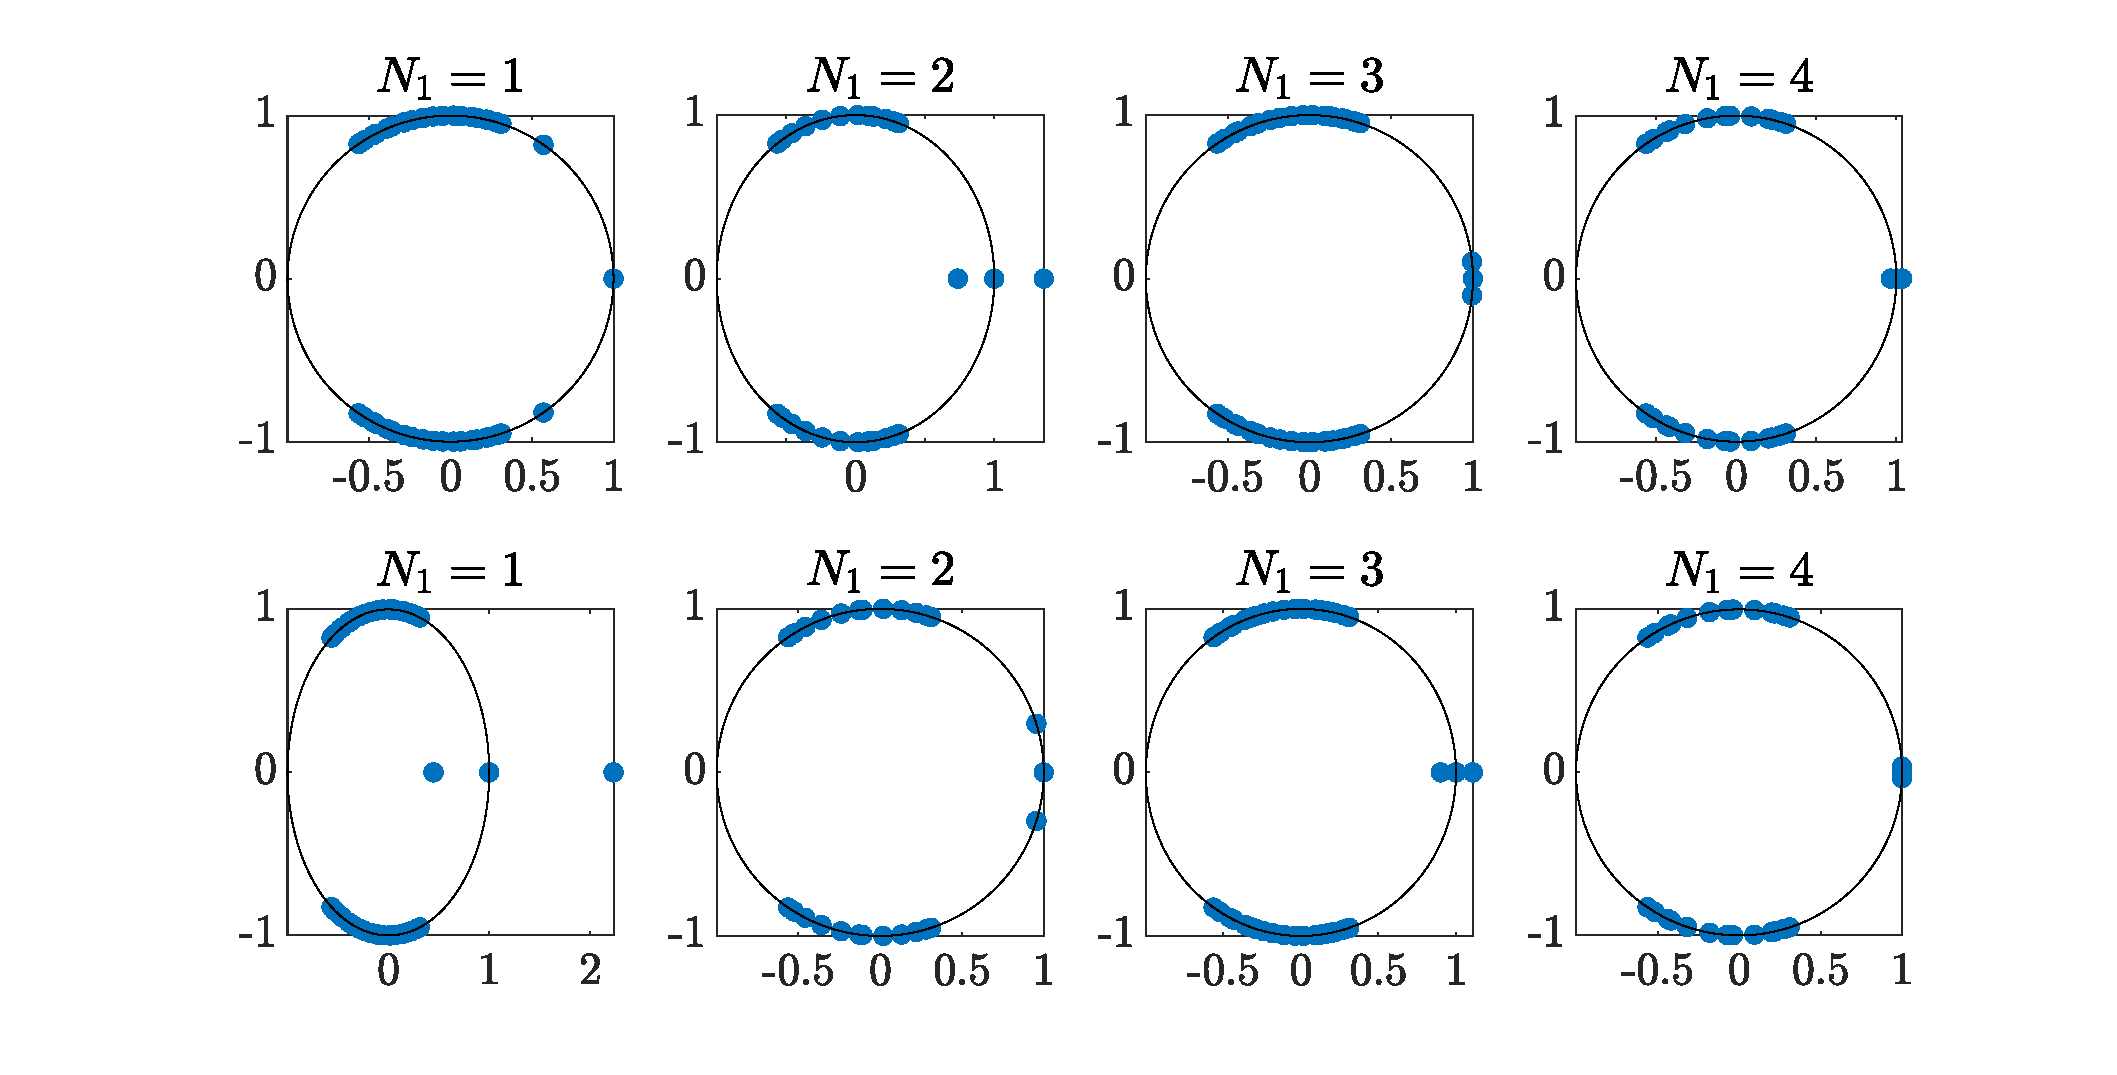
\includegraphics[width=15cm]{phi4hardfloqplot.eps}
	\caption{Floquet spectra for $N_1 = 1, 2, 3, 4$ for in-phase double breather (top) and out-of-phase double breather (bottom) for hard $\phi^4$ potential with $d = 0.125$.}
	\label{fig:phi4hardfloqplot}
\end{figure}

\cref{fig:bifdiagphi4} shows the bifurcation diagram for out-of-phase and in-phase double breathers for $N_1 = 6$. As noted above, the out-of-phase double breather is spectrally stable, while the in-phase double breather is unstable. For $N_1$ odd, this pattern is reversed (not shown). The upper branches are double breathers comprising two out-of-phase adjacent breathers, where we recall that this is the unstable configuration for the adjacent breather. The middle branch is an asymmetric double breather, comprising one single-site breather and one out-of-phase adjacent breather. \cref{fig:phi4eigerror} shows the relative error in the computation of the Floquet interaction eigenmodes on the lower branches for both the in-phase and out-of-phase double breathers for both even and odd $N_1$, using the formula \cref{eq:inteigsdouble}. As for the sine-Gordon equation, the relative error increases with $d$. We note that the relative error is less than $10^{-2}$ up to approximately $d = 3$, which is close to the turning points of the bifurcation diagrams. 

\begin{figure}
	\begin{center}
	\begin{subfigure}{0.3\linewidth}
		\caption{}
		\includegraphics[width=5.5cm]{phi4single.eps} \hspace{-0.5cm}
		\label{fig:phi4sola} 
	\end{subfigure}
	\begin{subfigure}{0.3\linewidth}
		\caption{}
		\includegraphics[width=5.5cm]{intersitephi4inphase.eps} \hspace{-0.5cm}
		\label{fig:phi4solb} 
	\end{subfigure}
	\begin{subfigure}{0.3\linewidth}
		\caption{}
		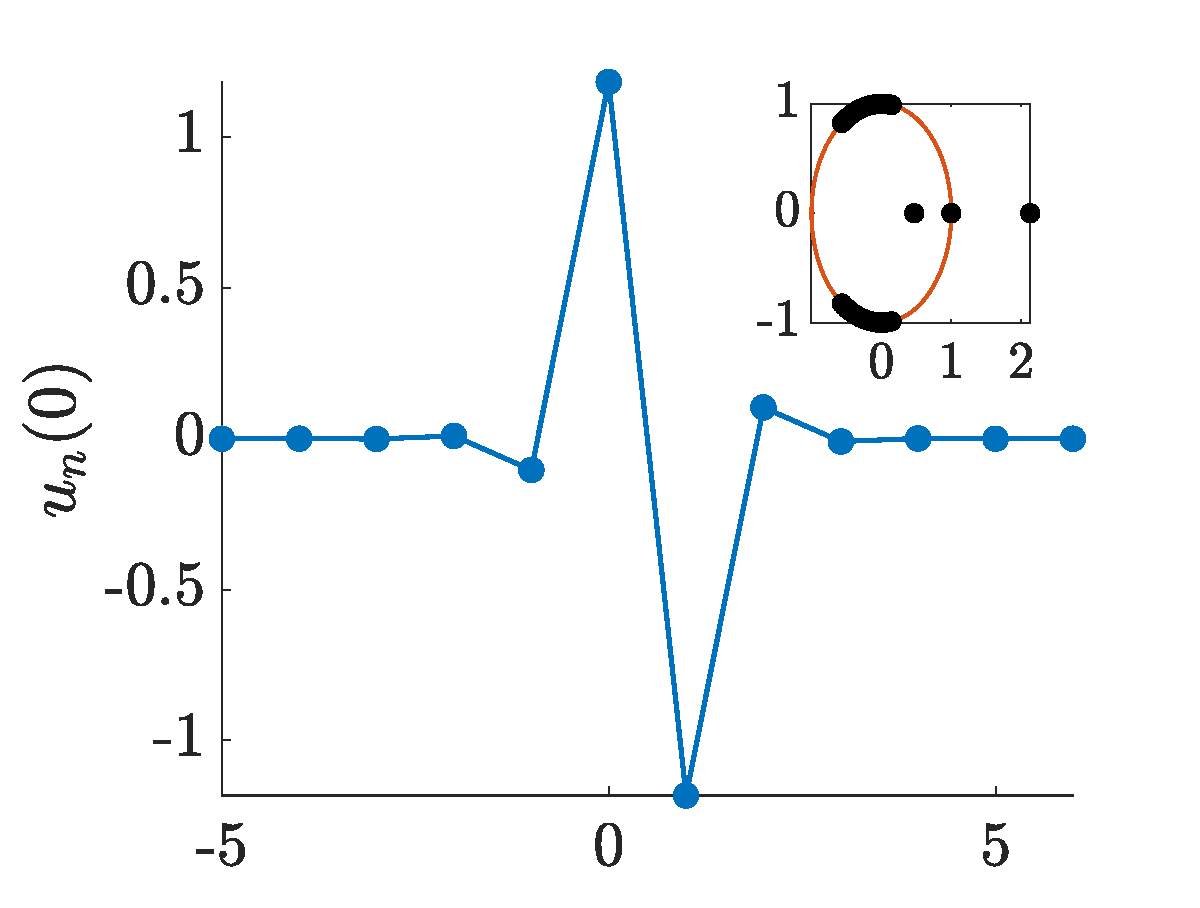
\includegraphics[width=5.5cm]{intersitephi4opposite.eps} 
		\label{fig:phi4solc} 
	\end{subfigure}
	\end{center}
	\caption{Initial condition $u_n(0)$ and Floquet spectrum (inset) for primary breather (a), in-phase adjacent breather (b), and out-of-phase adjacent breather (c) for hard $\phi^4$ potential with coupling parameter $d=0.1$. }
	\label{fig:phi4sol}
\end{figure}

\begin{figure}
	\hbox{
	\hspace{-2cm}
	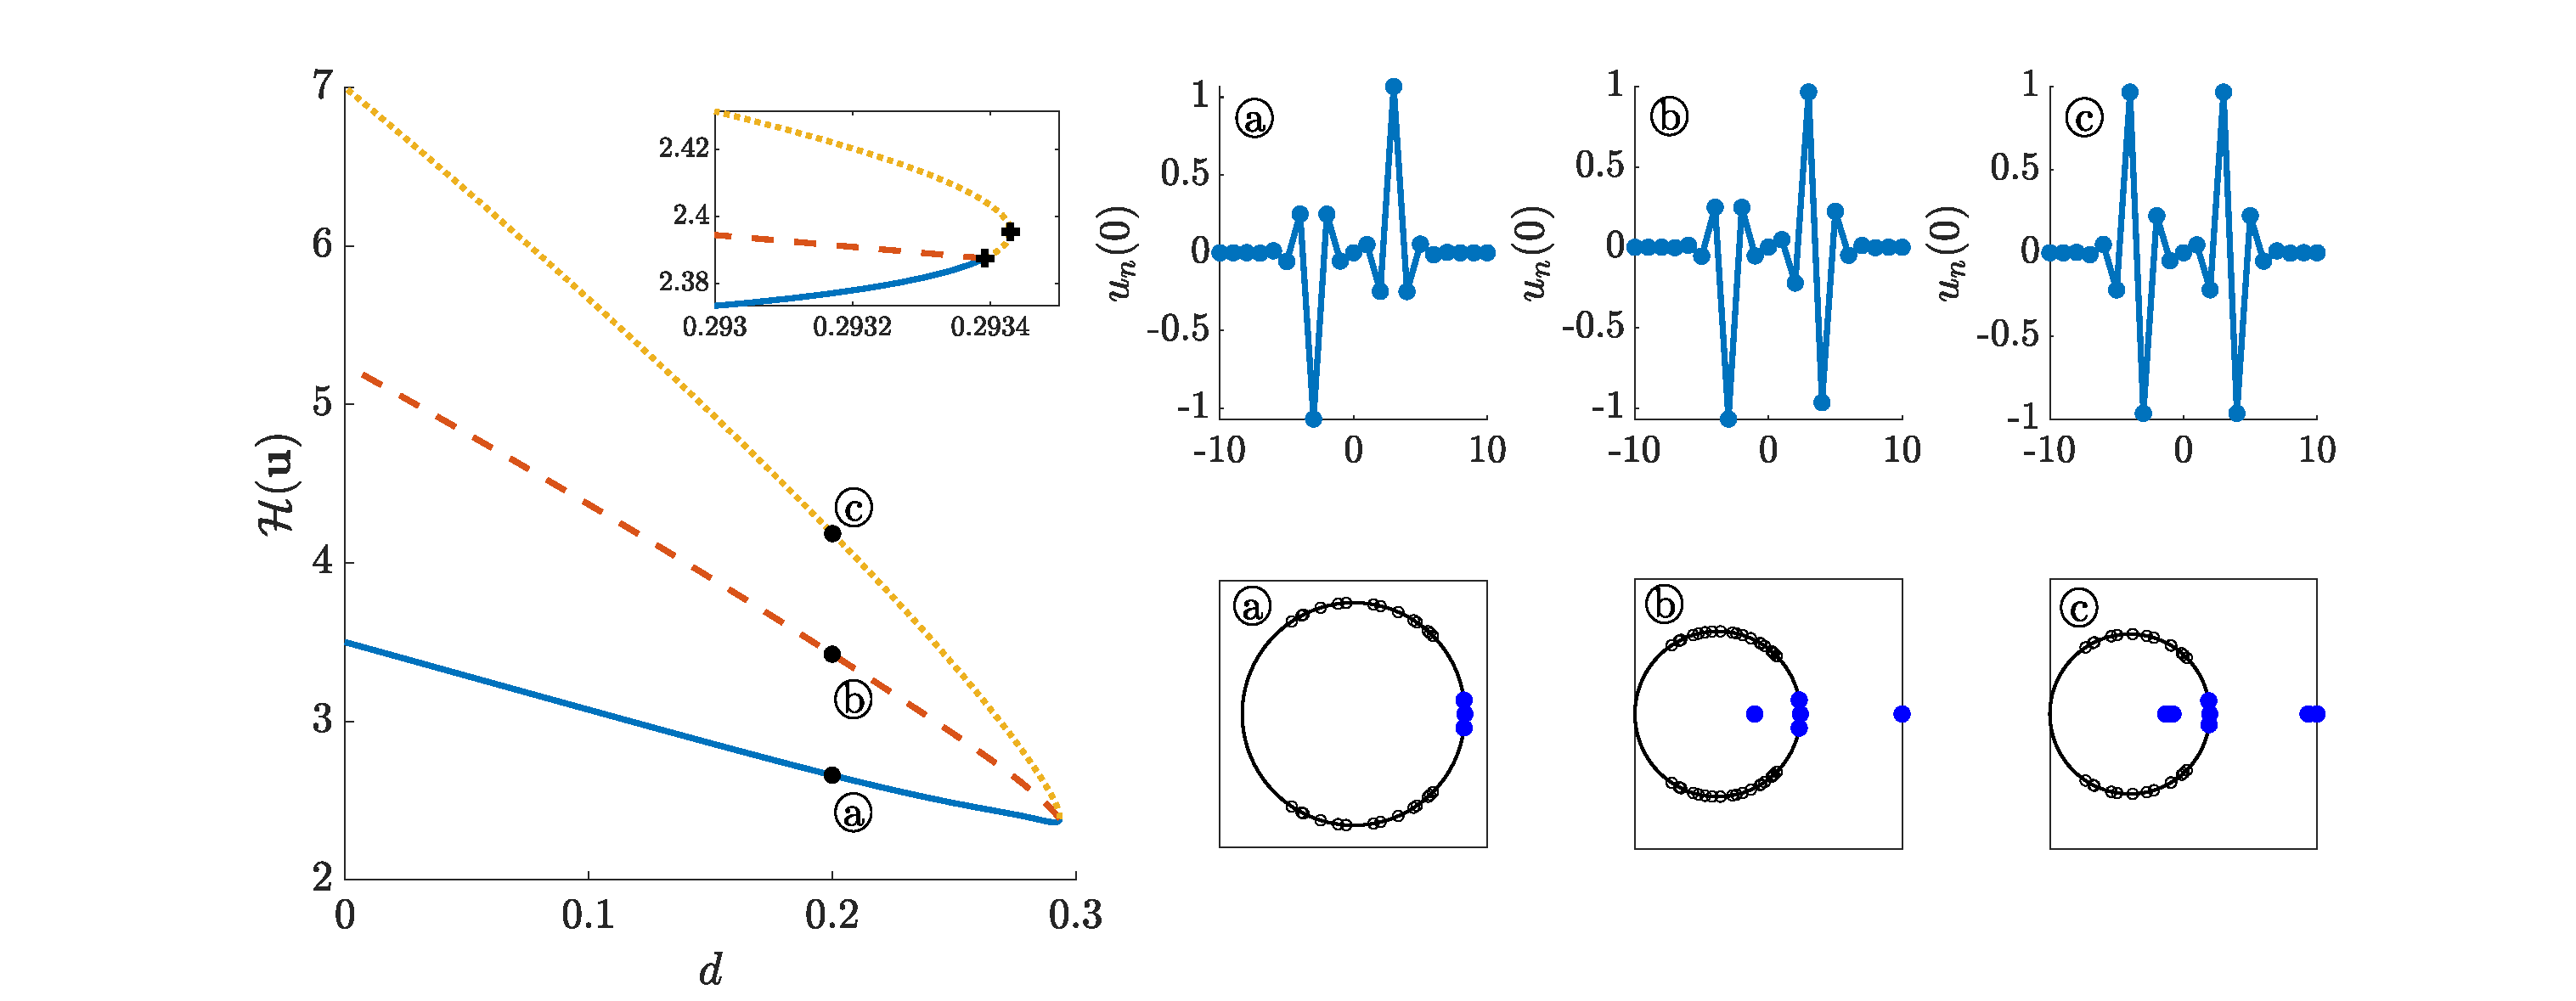
\includegraphics[width=20cm]{bifdiagphi4oppositeN6.eps}
	}
	\hbox{
	\hspace{-2cm}
	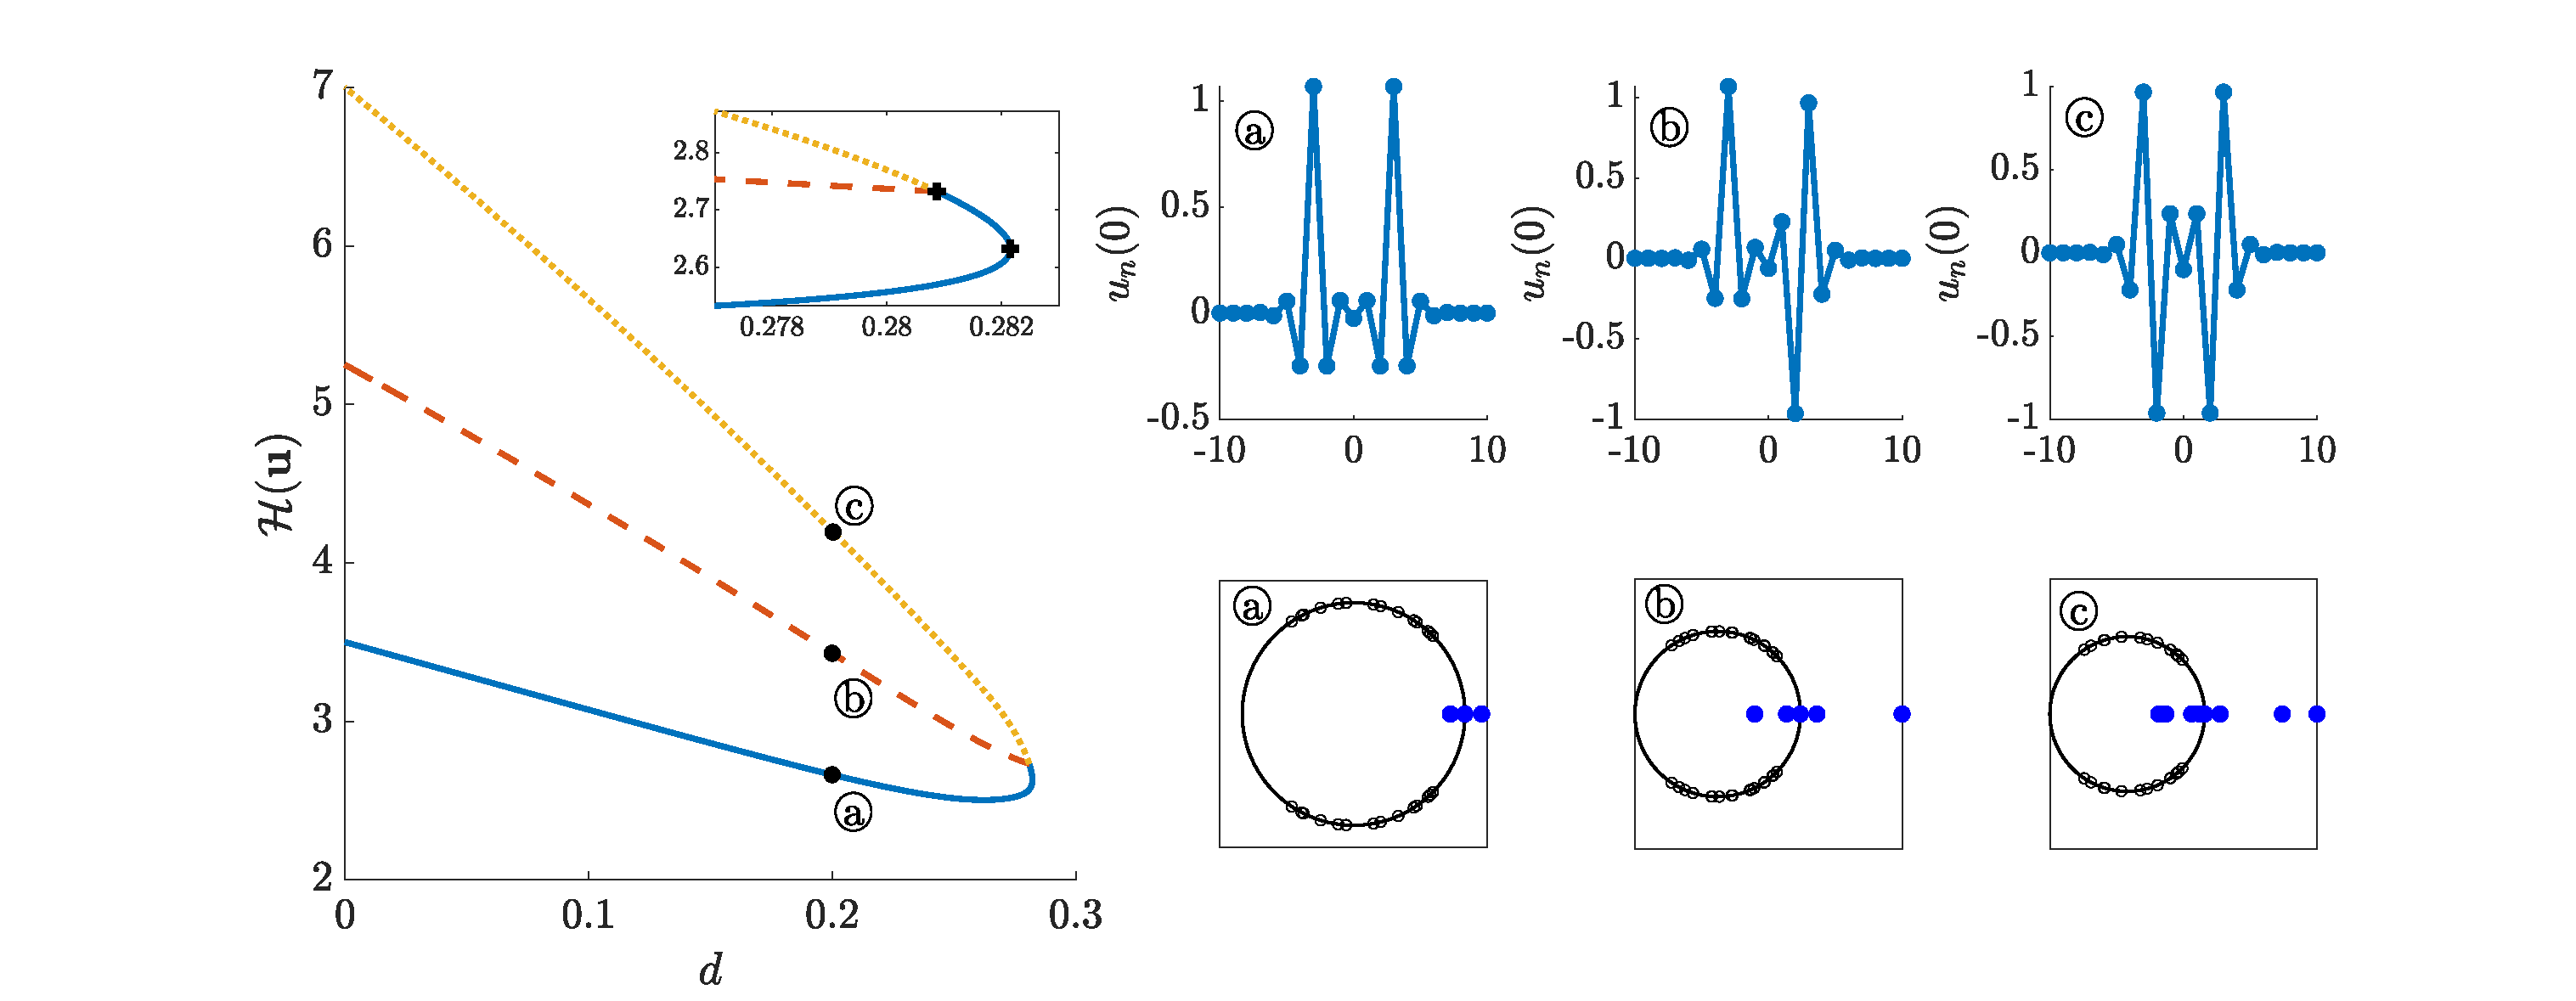
\includegraphics[width=20cm]{bifdiagphi4inphaseN6.eps}
	}
	\caption{Bifurcation diagram for hard $\phi^4$ potential for out-of-phase (top) and in-phase (bottom) double breather with $N_1 = 6$. Solutions and Floquet spectra on right correspond to labeled points on left.}
	\label{fig:bifdiagphi4}
\end{figure}

\begin{figure}
	\begin{center}
		\begin{subfigure}{0.45\linewidth}
		\caption{}
		\includegraphics[width=7.5cm]{images/doublephi4eigerrorpp.eps} 
		\label{fig:phi4eigerrora} 
	\end{subfigure}
	\begin{subfigure}{0.45\linewidth}
		\caption{}
		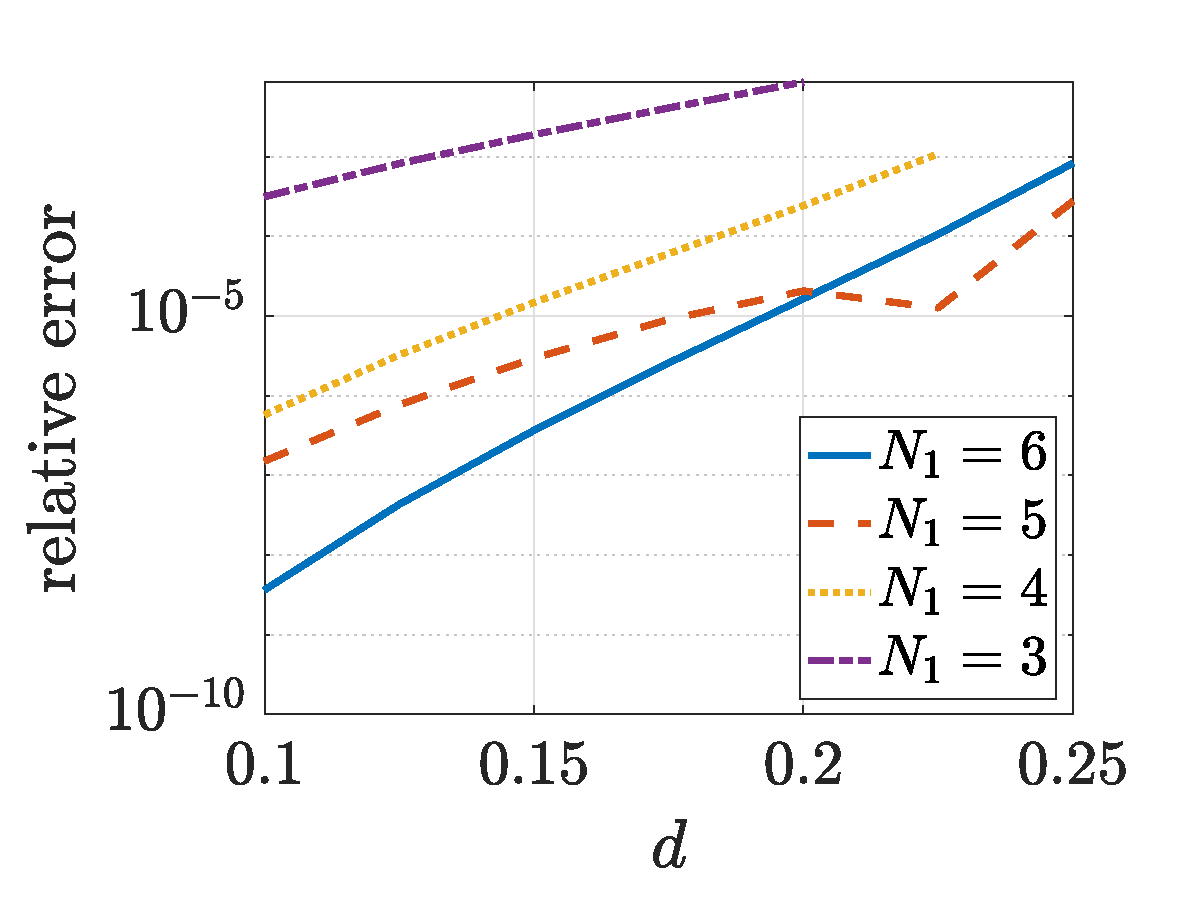
\includegraphics[width=7.5cm]{images/doublephi4eigerrorpm.eps} 
		\label{fig:phi4eigerrorb} 
	\end{subfigure}
	\end{center}
	\caption{Semilog plot of relative error of interaction eigenvalue computation vs. $d$ for in-phase (a) and out-of-phase (b) double breathers for hard $\phi^4$ potential with $N_1 = 3, 4, 5, 6$.}
	\label{fig:phi4eigerror}
\end{figure}

\section{Conclusions and future directions}

\paragraph{\textbf{Acknowledgments}}

This material is based upon work supported by the U.S. National Science Foundation under the RTG grant DMS-1840260 (R.P. and A.A.)
and DMS-1809074 (P.G.K.).

\appendix

\section{Proof of \texorpdfstring{\cref{th:spectrum}}{Theorem 2} }\label{app:specproof}

The proof is a straightforward adaptation of the proof of \cite{Parker2020}*{Theorem 2}. Let $Y(n) = (y(n), \tilde{y}(n)) = \omega \partial_\omega U(n)$. We take as an ansatz for the eigenfunction $W(n)$ the following piecewise linear combination
\begin{equation}\label{eq:Wansatz}
W_i^\pm(n) = c_i ( \dot{U}_i^\pm(n) + \lambda Y_i^\pm(n) ) + \tilde{W}_i^\pm(n),
\end{equation}
where $c_i \in \C$, and $W_i^\pm(n)$ is defined on the same interval as $U_i^\pm(n)$ in \cref{eq:Upiecewise}. Substituting \cref{eq:Wansatz} into \cref{eq:dynEVPM}, using the relations
\begin{equation}
\begin{aligned}
\dot{U}_i^\pm(n+1) &= DF_M(U(n))\dot{U}_i^\pm(n) \\ 
\qquad Y_i^\pm(n+1) &= DF_M(U(n)) Y_i^\pm(n) + 2 \partial_t B \dot{U}_i^\pm(n),
\end{aligned}
\end{equation}
and simplifying, we obtain the equation
\begin{equation}\label{eq:EVPpiecewise}
\begin{aligned}
\tilde{W}_i^\pm(n+1) &= DF(\sigma_i Q_M(n)) \tilde{W}_i^\pm(n) + \lambda^2 c_i B[ 2 \partial_t Y_i^\pm(n) + \dot{U}_i^\pm(n)] \\
&\quad+ [G_i^\pm(n) + (2 \lambda \partial_t + \lambda^2) B] \tilde{W}_i^\pm(n) + c_i \lambda^3 B Y_i^\pm(n),
\end{aligned}
\end{equation}
where
\begin{equation}\label{eq:Gipm}
G_i^\pm(n) = DF_M(U_i^\pm(n)) - DF_M(\sigma_i Q_M(n)).
\end{equation}
In addition to solving \cref{eq:EVPpiecewise}, the eigenfunction $W_i^\pm$ must satisfy matching conditions at $n = \pm N_i$ and $n = 0$. As in \cites{Parker2020,Parker2021,Sandstede1998}, this will in general not be possible. Instead, we solve the system 
\begin{equation}\label{eq:EVPsystem}
\begin{aligned}
\tilde{W}_i^\pm(n+1) &= DF(\sigma_i Q_M(n)) \tilde{W}_i^\pm(n) + \lambda^2 c_i B[ 2 \partial_t Y_i^\pm(n) + \dot{U}_i^\pm(n)] \\
&\quad+ [G_i^\pm(n) + (2 \lambda \partial_t + \lambda^2) B] \tilde{W}_i^\pm(n) + c_i \lambda^3 B Y_i^\pm(n) \\
\tilde{W}_i^+(N_i^+) &- \tilde{W}_{i+1}^-(-N_i^-) = C_i c \\
\tilde{W}_i^+(0) &- \tilde{W}_i^-(0) \in \C Z_M(n),
\end{aligned}
\end{equation}
where
\begin{equation}
\begin{aligned}
C_i c &= [ \dot{U}_{i+1}^-(-N_i^-) + \lambda Y_{i+1}^-(-N_i^-) ]c_{i+1} 
- [ \dot{U}_i^+(N_i^+) + \lambda Y_i^+(N_i^+) ] c_i.
\end{aligned}
\end{equation}
A solution to \cref{eq:EVPsystem} is an eigenfunction if and only if the $m$ jump conditions
\begin{equation}\label{eq:jump1}
\xi_i = \langle \sigma_i Z_M(0), \tilde{W}_i^+(0) - \tilde{W}_i^-(0) \rangle = 0
\end{equation}
are satisfied.

We proceed as in the proof of \cite{Parker2020}*{Theorem 2}. Since $DF(0)$ is hyperbolic, and $\| Q_M(n) \|_{L^2_\per([0,T])} \leq C r_M^{-|n|}$ by the stable manifold theorem, we can adapt the results of \cite{Palmer1988} to decompose the evolution operator $\Phi(m,n)$ of the variational equation \cref{eq:vareq} in exponential dichotomies on $\Z^\pm$. We then rewrite \cref{eq:EVPpiecewise} as a fixed point problem using the discrete variation of constants formula (see, for example, \cite{Parker2020}*{Lemma 3}), and project onto the stable and unstable subspaces of the exponential dichotomy. From there, we follow the steps in \cite{Parker2020}, using the estimates \cref{eq:Uestimates}, to obtain a unique solution to \cref{eq:EVPsystem}. The jump conditions \cref{eq:jump1} become
\begin{equation}\label{eq:jump2}
\begin{aligned}
\xi_i &= \sigma_i \sigma_{i+1} \langle Z_M(N_i^+), \dot{Q}_M (-N_i^-) \rangle (c_{i+1} - c_i) 
+ \sigma_i\sigma_{i-1} \langle  Z_1(-N_{i-1}^-), \dot{Q}(N_{i-1}^+) \rangle (c_i - c_{i-1}) \\
&\qquad -\frac{1}{d} \lambda^2 \sum_{n=-\infty}^\infty \left\langle Z_M(n+1), B[ 2 \partial_t Y(n) + \dot{Q}(n)]\right\rangle + R(\lambda)_i(c),
\end{aligned}
\end{equation}
where the remainder term has uniform bound
\[
\| R(\lambda)(c)\|_{X_M^2} \leq C \left( (r_M^{-N} + |\lambda|)^3\right).
\]
Evaluating the inner products, we obtain
\begin{equation}\label{eq:jump3}
\begin{aligned}
\xi_i &= a_i (c_{i+1} - c_i) + \tilde{a}_{i-1} (c_i - c_{i-1}) + \frac{1}{d} \lambda^2 M + R(\lambda)_i(c),
\end{aligned}
\end{equation}
where $a_i$ and $\tilde{a}_{i-1}$ are defined by \cref{eq:ai} and $M$ is defined by \cref{eq:M}. Equation \cref{Elambda} follows by writing the jump conditions \cref{eq:jump3} in matrix form as
\begin{equation}\label{eq:matrixform}
\left( A + \frac{1}{d} M \lambda^2 I + R(\lambda) \right) c = 0
\end{equation}
on $\R^m$, where $c = (c_1, \dots, c_m)^T$, and the matrix $A$ is defined by \cref{eq:matrixA}. Equation \cref{eq:matrixform} has a nontrivial solution if and only if its determinant is 0.

\bibliographystyle{amsplain}
\bibliography{DKG.bib}

\end{document}